%% pasner_thesis.tex 11/14/2018
%% Modified by Jacob M. Pasner
%% Copyright (C) 1988-2004 Daniel Gildea, BBF, Ethan Munson.
%
% This work may be distributed and/or modified under the
% conditions of the LaTeX Project Public License, either version 1.3
% of this license or (at your option) any later version.
% The latest version of this license is in
%   http://www.latex-project.org/lppl.txt
% and version 1.3 or later is part of all distributions of LaTeX
% version 2003/12/01 or later.
%
% This work has the LPPL maintenance status "maintained".
% 
% The Current Maintainer of this work is Daniel Gildea.

\documentclass[11pt]{ucthesis}
\def\dsp{\def\baselinestretch{2.0}\large\normalsize}
\dsp

% Declare usepackages here:
\usepackage{lineno}
\usepackage{color}   % May be necessary if you want to color links
\usepackage{hyperref} % Makes Chapter titles into links
\usepackage{amsmath}
\usepackage{bm}
\usepackage{caption,subcaption,epsfig}
\hypersetup{
  colorlinks=true, % set true if you want colored links
  linktoc=all,     % set to all if you want both sections and subsections linked
  citecolor=black,
  filecolor=black,
  linkcolor=black, % choose some color if you want links to stand out
  urlcolor=black
}

\linenumbers

\setlength{\parindent}{0pt} % no indentation
\setlength{\parskip}{2ex} % larger space between paragraphs

% Definitions for using atlas latex
\newcommand*{\ATLASLATEXPATH}{atlaslatex/latex/}
\usepackage[jetetmiss,particle,misc]{atlaslatex/latex/atlasphysics}
\usepackage[backend=biber,sorting=none,backref=true]{biblatex}

% Define biliography resources for lookup by biber
\addbibresource{atlaslatex/bib/ATLAS-useful.bib}
\addbibresource{atlaslatex/bib/ATLAS-errata.bib}
\addbibresource{atlaslatex/bib/ATLAS.bib}
\addbibresource{atlaslatex/bib/CMS.bib}
\addbibresource{atlaslatex/bib/ConfNotes.bib}
\addbibresource{atlaslatex/bib/PubNotes.bib}
\addbibresource{pasner_thesis.bib}


\begin{document}

% Declarations for Front Matter

\title{An Inclusive Search for the decay of a Boosted Higgs boson in the $H
\rightarrow$ \MakeLowercase{$b\overline{b}$} channel with the ATLAS detector}
\author{Jacob Martin Pasner}
\degreeyear{2019}
\degreemonth{October}
\degree{DOCTOR OF PHILOSOPHY}
\chair{Professor Jason Nielsen}
\committeememberone{Professor Abraham Seiden}
\committeemembertwo{Professor Michael Hance}
\numberofmembers{3} %% (including chair) possible: 3, 4, 5, 6
\deanlineone{Dean Lori Kletzer}
\deanlinetwo{Vice Provost and Dean of Graduate Studies}
\deanlinethree{}
\field{Particle Physics}
\campus{Santa Cruz}

\begin{frontmatter}

\maketitle
\copyrightpage

\tableofcontents
\listoffigures
\listoftables

\begin{abstract}

A search for high-momentum Higgs bosons, produced with an associated jet and
decaying to bottom quark pairs, is conducted using an integrated luminosity of
$80.5~\ifb$ of proton-proton collisions at $\sqrt{s} = 13~\TeV$ collected
with the ATLAS detector at the Large Hadron Collider.  The search for $H
\rightarrow b\bar{b}$ is of particular importance, as current measurements of
this decay channel contain large uncertainties and have not yet established
evidence for the gluon-gluon fusion and vector boson fusion Higgs boson
production modes. This is the first time this analysis has been performed with
$\sqrt{s} = 13~\TeV$ at ATLAS and represents an important advancement in the use
of boosted jet techniques including implementation of the Variable Radius jet
algorithm.  Furthermore, a novel $t\bar{t}$ control region strategy is
implemented to correct the mismodeling of its normalization and is shown to
constrain the associated large JES and JMR systematic uncertainties. For the
Standard Model Higgs boson, the observed signal strength is $\mu_{H} = 5.8 \pm
3.1~\mathrm{(stat.)} \pm 1.9~\mathrm{(syst.)} \pm 1.7~\mathrm{(theo.)}$, which
is 1.6 standard deviations higher than the background-only hypothesis, with an
expected sensitivity of $0.28\sigma.$


\end{abstract}

\begin{dedication}
\null\vfil
{\large
\begin{center}
Dedication\\\vspace{12pt}
Dedication\\\vspace{12pt}
Dedication
\end{center}}
\vfil\null
\end{dedication}


\begin{acknowledgements}

\label{sec:acknowledgements}

There is no way I can fully express my gratitude for the people and places that
have made this journey all that it has been.  The path to this degree has been
winding, uncertain and full of mistakes.  The names below represent a small
sample of the rich bounty this life has offered me for guidance and support. I
am eternally grateful to them all.

Thank you Jason Nielsen for personally calling me and inviting me to work with
you nearly seven years ago.  I didn't know how lucky I was back then, but I can
definitively say now I wouldn't have it any other way.  Your patience,
exuberance, curiosity and kindness have taught me the power of questions and
the boundless possibilities of an inquisitive mind. Thank you for these gifts,
and for supporting me in the pursuit of my dreams.

Thank you to my committee members, Michael Hance and Abraham Seiden, for
bearing with the hectic timeline this dissertation was created on.  You
supported my less than traditional writing style and have helped me produce a
document  my family and I can be proud of for years to come.

Thank you to my collaborators in ATLAS and all my individual analysis groups.
It has been an incredible honor to work with such a diverse and devoted group
of brilliant scientists.  Our incredible success as a field stands as a
testament to the ingenuity and determination that can only come from
cooperation.  Particle physicists have shown me what a world without boarders
looks like, and I am grateful to count myself amongst their ranks.

Thank you to the teachers and professors who helped me realize my dream of
becoming a scientist and more: Richard Toothman, John McDaniel (McD), Kelley
Molitor, Mani Tripathi, Manuel Calder\'on de la Barca S\'anchez, Randy Harris,
and Joel Primack.  You believed in me and I will never forget the power of that
gift.

Thank you to Giordon Stark for seeing my potential and setting me on the path
to policy.  You have been a solid shoulder to lean on, a kind ear (eye?) to my
worries and a powerful mind to sharpen my own against. Your friendship and
brilliance make this world more friendly and interesting, everywhere you go.
Also your baking is so good it should come with a warning label.

Thank you to the many post doctoral students at UCSC who have pulled me out of
the academic mud time and time again: Matthew, Andrea, Simone, Hass, Chiara and
Ryan.  Navigating the ATLAS collaboration without your guidance and protection
seems an impossible task, we are all in your debt.

Thank you to my physics cohort for all the late night homework sessions and
your continuing friendship and support: Joey, Max, Ross, Dean, Cam, Mike, Dave,
Noah, Peizei, Ahram, Skyler, Christoph, Eudald, Daniel, Philip.  You're all
brilliant and I can't wait to see where life takes you all. 

Thank you to the UCSC graduate students who helped me along the way, sometimes
with words of encouragement, other times with a stiff drink but always with a
smile: Sheena, Peyton, Eric, Jeff, Alexander, Monika, Carey, Doug, Brian,
Muiris, Daniel, Jerah, Katie, Tayler, Daniel, Zippy, Carolyn, Cole, Natasha and
many more.  Graduate school is hard in a way very few people can understand,
I'm so glad I didn't have to travel this path alone, thanks to you.

Thank you to my Santa Cruz housemates through the years: Elizabeth, Tessa,
Stas, Dave, David, Rob, Roy, Zad, Brent, Philip, Graham, Kelly and Catherine.
The house on Laurel Street will always be a special place in my memories and my
heart.  The music, food, dance and discussion we shared have taught me what
true community looks like.  My love and gratitude to all of you, I couldn't ask
for better or more supportive friends.

Thank you to the Santa Cruz locals for all the shenanigans and
memories: Cleveland, Gabe, Monica, Travis, Saul, Bob, Larry, Deidre, Brian,
Philip, Sean, Lance, Chappy, Keelin, Angelica, Kage, Mikey (thanks for the
laundry), Michael, Micha, Xander, Gabriel, Julian, Brooke, Maya, Rafferty,
Allie, Sam, Kate, Carrie, Alex, Cesar, Nora, Chris and many more. Our time
together gave me the moments of rest and relaxation I needed to keep me sane.

Thank you to my Geneva housemates during my time in Switzerland: Rob, Bijan,
Leigh and Jennifer.  Living abroad was scary and hard until you welcomed me
into the Marigold Memory Palace and your hearts.  Here's to the future and our
continued friendship. 

Thank you to everyone who made my time living abroad an exciting and eye
opening experience: Fenton, Paolo, Ivan, Marika, Niko, Oliver, Ranveig,
Tristan, Apostolos, Efi, Irene, Leo, Arizona, Soph, Elsa, Adrian, George,
Kelvin, Dayane, Enrica, Sam, Galen, Kisa, Babette, Viktoria, Adam, Sam, Joel,
Amal, Danii, Flavia, Julie, Cameron, Mor, Swathi, Gabriella (Biscoitinha),
Duncan, Eddie, Murdo, Lewis, Stoyan, Sophie, Sun, Xanthe, the entire LTA,  and
many more.  Together we danced, hiked, boxed, ran, snowboarded, flew, sailed,
biked and rode our way through more adventures than I'd ever thought possible.
My life is so much richer thanks to you.

Thank you to Josh and Emmanuel for putting up with having a crazy particle
physicist as the intern for 10 weeks.  You gave me the foot in the door I
needed to set off on the next stage of my life in policy.  Next round of coffee
is on me.

Thank you to Heidi for being there for me in what has been the most trying
period of my life thus far.  You saw me through Giardia, injuries and crippling
writing stress.  Whatever life brings us, I am lucky to have had your strength
during this time. 

Thank you to Vin for seeing me through the lowest lows and the highest highs.
You've done more for me than words can describe.  I treasure your friendship
and will always love you.  Here's to our next adventure!

Thank you to my sister Yara for being my best friend.  I can talk to you about
anything, from group theory to relationships to politics and always appreciate
your advice.  I can't wait to see what you do in this world and am thankful to
have you in my life, love you moo moo.

Thank you to my parents Mike and Izzy.  You gave me life, you fostered my
imagination, and have bent over backwards to support my dreams.  All of my
accomplishments, all of my life, I owe in some part to you and your example. My
love and gratitude towards you knows no bounds and will exist as long as I'm
living.

Thank you to music for giving me a way to express myself when nothing made
sense.  In my times of greatest need I have found strength in your ethereal
arms. A special thanks to the local Irish session, all my Lark friends and
Nathaniel Berman and his concert choir and wind ensemble.

Thank you to science for giving me the tools to answer my never ending
questions.  You have given me the lens I needed to make sense of this world,
and my what a beautiful world it is. 

And finally, thank you to the Earth for giving us such a beautiful, bountiful
and rich place to call home.


\end{acknowledgements}

\end{frontmatter}


\chapter{Introduction} \label{sec:intro}
As children we are fascinated with the natural world that surrounds us.  How
was it made? What is it made of? Where did it come from?  When was it made?
These questions follow some of us into adulthood and lead to the study of the
fundamental interactions of the Universe, the pursuit of the building blocks of
reality.  For the past century, experiments of increasing size and complexity
have probed higher energies and smaller distances to answer these questions out
of the pure desire to know the unknown.  The results of these experiments have
been interpreted and used to build the most predictive and successful theory
across all of science - the Standard Model (SM) of particle physics. At the
current state-of-the-art facility, the Large Hadron Collider (LHC), an
international team of scientists and engineers continue this legacy of
discovery.  There, protons are smashed together at energies not seen since the
birth of the Universe some 13.8 billion years ago and the results are analyzed
to answer the outstanding questions of our time.

In 2012 the discovery of a Higgs-like boson \cite{Higgs:1964ia, Higgs:1964pj,
Higgs:1966ev, Englert:1964et, Guralnik:1964eu} at CERN by the ATLAS and CMS
\cite{Aad:2012tfa,Chatrchyan:2012xdj} collaborations answered one of these
outstanding questions, namely: What is the origin of mass for particles in the
SM?  This was a major triumph for both the theoretical and experimental
particle physics communities and resulted in the Nobel Prize in Physics being
awarded to Francois Englert and Peter W. Higgs for their contributions to the
Brout-Englert-Higgs theory. However, the properties of this new particle are
still under verification, and new physics could be lurking in the large
uncertainties of current observations of the SM Higgs boson.  In particular,
the coupling strength of the Higgs boson to bottom quarks ($H \rightarrow
b\bar{b}$) was only observed in 2018, and the measurement still has a large
uncertainty \cite{HIGG-2018-04, CMS:2018abb}. Furthermore, the $H \rightarrow
b\bar{b}$ decay mode has yet to be observed for the vector boson fusion and
gluon-gluon fusion production mechanisms.  Finally, new physics could be
accessible through observation of highly boosted Higgs bosons produced via
gluon-gluon fusion, which is sensitive to possible anomalous couplings in the
top-quark loop \cite{Grojean:2013nya, Schlaffer:2014osa}.  Thus, this analysis
aims to directly measure the coupling of the Higgs boson to bottom quarks,
focusing on the observation in the gluon-gluon fusion and vector boson fusion
production modes. 

\Cref{part:theory} of this dissertation describes the Standard Model of
particle physics including the Higgs mechanism and motivates the search for
highly boosted $H \rightarrow b\bar{b}$ production and decay.
\Cref{part:experiment} describes both the LHC and the ATLAS detector located at
CERN. Lastly, \Cref{part:HbbISR} presents the analysis and the boosted
Higgs boson measurement results.


\part{Theoretical Motivations and the Standard Model}
% The Standard Model and Beyond

\chapter{The Standard Model and Beyond} \label{chap:standard_model}

\section{The Standard Model} \label{sec:theory:standardmodel}

At the turn of the 20th century our understaning of the constituent matter of
the universe was limited to what we could see with microscopes and imply from
the observations of light and elctricity, giving us evidence for both the photon
and the electron.  In the first half of the century we discovered the field of
subatomic physics with Rutherfords 1911 gold foil scattering experiment, and
Dirac successfully demonstrated the quantization of the electromagnetic field,
the first step towards a fully Gauge Invariant Quantum Field Theory.
In the second half we literally delved deeper, discovering that the nucleus
contained structure and extended our theories to include the the complex
mechanics of quarks and gluons.  With the discovery of the Higgs in 2013 the
Standard Model has become an irrefutable framework as can be seen in the high
level of agreement betwee theory experiment in figure \ref{fig:comparison}.

\begin{figure}[!htbp]
  \begin{center}
    \includegraphics[width=0.8\linewidth]{figures/atlas/muon_system}
    \caption{ \cite{PERF-2007-01} A cut-away diagram of the ATLAS muon system
and its many sub-detectors.}
    \label{fig:muon_system}
  \end{center}
\end{figure}

The QCD and QED theories predict two classes of particles: fermions and
bosons. These particles represent the quanta of the quantum fields of the
Standard Model and and the mediators of the fundamental forces of Nature.


\section{Quantum Chromodynamics} \label{sec:theory:qcd}

Quantum Chromodynamics is the continuation of the mathematical framework
established by the electroweak formalism in \Cref{sec:theory:gsw}, this time
for the strong force described by the $SU(3)_C$ gauge group, where $C$
represents the ``color" charge of QCD \cite{Campbell:2017hsr}.  This
color charge doesn't imply actual visible color, but is useful as an analogy to
the visible spectrum where a combination of red, green, and blue generates
white.  For QCD the combination of red, green, and blue color charges can
result in a colorless object.  As mentioned in \Cref{sec:theory:fermions}, the
quarks have a color (anti-color) charge defining color triplet field which
transforms under the general $SU(3)$ transformation as

\begin{equation}
q = \left( \begin{matrix} q_{r} \\ q_{g} \\ q_{b} \end{matrix} \right)
\rightarrow q^{'} = exp \left( ig_{s} \sum_{k=1}^{8} \eta_{k}(x)
\frac{\lambda_k}{2} \right) q
\end{equation}

Here the $\lambda_{k}$ are the Gell-Mann generators for $SU(3)$, $\eta(x)_{k}$ is the
space-time dependency for each generator, and  $g_s$ is the strong coupling constant.
As with the electroweak Lagrangian, the introduction of these space-time dependent terms adds new
terms into the kinematic portion of the Lagrangian and spoils the gauge 
invariance.  Again, a covariant derivative is introduced 

\begin{equation}
D_{\mu} = \partial_{\mu} - ig_{s}G_{\mu}^{k}\frac{\lambda_{k}}{2}
\end{equation}

to restore gauge invariance. The $G_{\mu}^{k}$ are the new fields introduced
for the 8 gluons.  These new fields transform under $SU(3)$ as

\begin{equation} \label{eq:qcd:gluon_field}
G_{\mu}^{k} \rightarrow G_{\mu}^{'k} = G_{\mu}^{k} + \partial_{\mu}\eta_{k}(x) +
g_{s}f_{klm}\eta_{l}(x)G_{\mu}^{m}
\end{equation}

Given these definitions the QCD Lagrangian ($\mathcal{L}_{QCD}$) can be
constructed as 

\begin{equation} \label{eq:qcd:qcd_lagrangian}
\mathcal{L}_{QCD} = \bar{q}(i\gamma_{\mu}D^{\mu} - m_{q})q -
\frac{1}{4}G_{k}^{\mu\nu}G_{k\mu\nu}
\end{equation}

where the gluon field tensor $G_{k}^{\mu\nu}$ is defined as

\begin{equation} \label{eq:qcd:gluon_tensor}
G_{k}^{\mu\nu} = \partial^{\mu}G_{k}^{\nu} - \partial^{\nu}G_{k}^{\mu} +
g_{s}f_{klm}G_{\l}^{\mu}G_{m}^{\nu}.
\end{equation}

The strong force is peculiar in that experiments observe only colorless objects
in the form of bound states of quarks known as hadrons.  Qualitatively, the
potential between quarks in a bound state (meson or baryon) gets stronger with
separation, unlike the other forces.  At the point where the system would
separate into color-charged objects, it becomes energetically favorable to
produce a quark/anti-quark pair in a process known as hadronization.  In other
words, attempting to separate a bound quark state into its colored constituents
simply results in new colorless bound states.  This requirement of colorless
objects by the strong force is known as color confinement. For highly energetic
strong interactions at hadron colliders the result is an expanding chain of
hadronizing quarks and gluons and their decay products known as a jet.


\section{Quantum Electrodynamics} \label{sec:theory:qed}

In the SM the Electromagnetic and Weak nuclear forces are unified into the
Electroweak interaction which is represented by the $SU(2)_L \times U(1)_Y$
gauge group. The L represents the physical observable that the Weak interaction,
and thus the $SU(2)$ transformation, only acts on left handed particle states.
The Y states that this is the $U(1)$ symmetry for the weak hypercharge Y instead
of the electromagnetic charge.  The particle states for these interactions are
solutions to the Dirac equation and are represented as Dirac spinor doublets
($\boldsymbol{\Psi_L}$) for the left handed states, and as Dirac spinor singlets
($\Phi_R$) for the right handed states.  Thus when a general transformation from
the Electroweak gague group is applied to the left handed spinor doublet you get
equation \ref{eq:qed:doublet}

\begin{equation} \label{eq:qed:doublet} 
\boldsymbol{\Psi_L} \rightarrow \boldsymbol{\Psi_L}^{'} = exp \left(
\underbrace{ ig^{'} \frac{Y_L}{2}
\zeta (x) }_{U(1)_Y} + \underbrace{ ig_{W} \boldsymbol{\alpha}(x) \cdot
\text{\bf{T}} }_{SU(2)_L} \right) \boldsymbol{\Psi_L}.
\end{equation}

For the right handed spinor singlet the $SU(2)_L$ doesn't contribute and
you get equation \ref{eq:qed:singlet}

\begin{equation} \label{eq:qed:singlet} 
{\Phi_R} \rightarrow \Phi_R^{'} = exp \left( \underbrace{ ig^{'} \frac{Y_R}{2}
\zeta (x) }_{U(1)_Y} \right) \Phi_R.
\end{equation}

We can see that these local gauge transformations have introduced space-time
depended terms $\boldsymbol{\alpha}$ and $\zeta$ into our electroweak
Lagrangian.  Due to the derivatives contained within the kinetic term of this
lagrangian, this new configuration would introduce additional terms, thus
violating our required local gauge invariance.  Luckily, we can remove these
additional terms by replacing the standard derivative ($\partial_{\mu}$) with th
covariant derivative ($D_{\mu}$) as seen in equation \ref{eq:qed:left} for the
left handed states and \ref{eq:qed:right} for the right handed states.

\begin{equation} \label{eq:qed:left} 
D_\mu = \partial_{\mu}
- \underbrace{\frac{1}{2}ig^{'}B_{\mu}Y_{L}}_{U(1)_Y} -
  \underbrace{\frac{1}{2}ig_{W}\bf{W}_\mu \cdot \boldsymbol{\tau}}_{SU(2)_L}
\end{equation}

\begin{equation} \label{eq:qed:right} 
D_\mu = \partial_{\mu}  - \underbrace{\frac{1}{2}ig^{'}B_{\mu}Y_{R}}_{U(1)_Y} 
\end{equation}

Here we see two new gauge fields; $B_\mu$ the weak hypercharge field and
$\boldsymbol{W_\mu}$ the charged weak field.  The form of these fields is chosen
such that the final Lagrangian is invariant under $SU(2)_L \times U(1)_Y$
transformations, and thus we have restored gauge invariance for the kinetic term
of our electroweak Lagrangian!  Inserting these new definitions into the
Lagrangian for the spinor field $\Psi$ which satisfies the free-particle Dirac
equation we get

\begin{equation} \label{eq:qed:lagrangian}
\mathcal{L} = i\bar{\boldsymbol{\Psi_L}}\gamma^{\mu} \left( \partial_{\mu}
- \frac{1}{2}ig^{'}B_{\mu}Y_{L} - \frac{1}{2}ig_{W}\bf{W}_\mu \cdot
  \boldsymbol{\tau} \right) \boldsymbol{\Psi_L} + i \Phi_{R}\gamma^{\mu}
\left(\partial_{\mu} - \frac{1}{2}ig^{'}B_{\mu}Y_{R} \right) \Phi_{R}
\end{equation}

Wavefunction
Transformation
Covariant Derivative
Lagrangian
Identify Terms

In the SM the electromagnetic and weak nuclear forces are unified into the
electroweak interaction which . . . 

Quantum Electrodynamics is the first model created in the QFT image.

\section{Spontaneous Symmetry Breaking} \label{sec:theory:ssb}

Spontaneous symmetry breaking occurs when a system loses an inherent symmetry in
order to attain a lower energy configuration.

\section{The Higgs Mechanism} \label{sec:theory:higgs}

The Higgs mechanism is the system by which the gauge bosons and fermions gain
mass through the spontaneous breaking of the electroweak symmetry of the Higgs
potential \cite{Higgs:1964ia,Higgs:1966ev,Thomson:2013zua}.  This section will
also discuss briefly the couplings of the Higgs boson to massive particles, as
well as its self couplings.

\subsection{Electroweak Symmetry Breaking}

The Higgs field is expressed as a complex doublet, $\boldsymbol{\Phi}$, and thus
has four components defined as

\begin{equation} \label{eq:higgs:higgs_field}
\boldsymbol{\Phi}(x) = \left( \begin{matrix} \phi^{+} \\ \phi^{0} \end{matrix}
\right) = \frac{1}{\sqrt{2}} \left( \begin{matrix} \phi_{1}(x) + i\phi_{2}(x) \\
\phi_{3}(x) + i\phi_{4}(x) \end{matrix} \right).
\end{equation}

The four components of this field each represent a degree of freedom which
become the longitudinal polarizations of the $W^{\pm},Z$ gauge bosons and the
Higgs boson.  The resulting Lagrangian for the Higgs includes a kinetic term
(K) as well as the Higgs potential (V), all of which are invariant under the
electroweak gauge symmetry $SU(2)_L \times U(1)_Y$.  The definition is

\begin{equation} \label{eq:higgs:lagrangian}
\mathcal{L}_{\text{Higgs}} =
\underbrace{(D_{\mu}\boldsymbol{\Phi)^{\dagger}}D^{\mu}\boldsymbol{\Phi}}_{\text{K}}
- (\underbrace{\mu^{2}\boldsymbol{\Phi}^{\dagger}\boldsymbol{\Phi} +
  \lambda(\boldsymbol{\Phi}^{\dagger}\boldsymbol{\Phi})^{2}}_{\text{V}}).
\end{equation}

Here the $\mu^{2} < 0$ and $\lambda > 0$ are constrained such that the
potential forms a ring stable minima.  The shape of this potential is shown in
\Cref{fig:higgs_potential} and is often described as the ``Mexican-hat" or
"wine-bottle" potential. 

\begin{figure}[!h]
  \begin{center}
    \includegraphics[width=0.4\linewidth]{figures/theory/higgs_potential.png}
    \caption{ A lower-dimensionality representation of the shape of the Higgs
potential.  The central peak represents a rotationally symmetric
unstable state, while the trough represents the infinite number of minima that
can be selected upon the spontaneous breaking of the symmetry.}
    \label{fig:higgs_potential}
  \end{center}
\end{figure}

The value of this minima can be calculated by taking the derivative of V with
respect to $\boldsymbol{\Phi}$ and setting it equal to $0$. This value, also
known as the vacuum expectation value (vev) has been found to be $v \equiv
\sqrt{-\mu^{2}/\lambda} = 246$ GeV. The arbitrary vev of the ground state Higgs
field is acquired when the symmetry of the Higgs potential is spontaneously broken.
For ease of calculation the coordinate system is oriented such that

\begin{equation}
\left\langle \boldsymbol{\Phi}(x) \right\rangle = \frac{1}{\sqrt{2}} \left(
\begin{matrix} 0 \\ v \end{matrix} \right)
\end{equation} 

Next small perturbations around the minimum of the Higgs
potential are parameterized as 

\begin{equation} \label{eq:higgs:broken_higgs}
\left\langle \boldsymbol{\Phi}(x) \right\rangle = \frac{1}{\sqrt{2}} \left(
\begin{matrix} 0 \\ v + h(x) \end{matrix} \right) \text{exp} \left(
i\frac{\tau^{i}}{2}\theta^{i}(x) \right)
\end{equation} 

Here the real scalar field $h(x)$ corresponds to radial perturbations of the
minima, and the three $\theta^{i}(x)$ are the Nambu-Goldstone fields with
values determined by the choice of gauge.  Choosing the unitary gauge of
$\theta^{i}(x) = 0$ and expanding the kinetic term of
\Cref{eq:higgs:lagrangian} around the vev gives

\begin{equation} \label{eq:higgs:boson_masses}
\mathcal{L}_{\text{Higgs},K} = \frac{g^{2}v^{2}}{8} \left(
(W_{\mu}^{-})^{\dagger}W^{-\mu} + (W_{\mu}^{+})^{\dagger}W^{+\mu} \right) +
\frac{1}{2} \left( \begin{matrix} W_{\mu}^{3\dagger} & B_{\mu}^{\dagger}
\end{matrix} \right) \boldsymbol{M}^{2} \left( \begin{matrix} W^{3\mu} \\ B^{\mu}
\end{matrix} \right) + \ldots 
\end{equation}

Here the first term is the physical mass term for the $W^{\pm}$ bosons where
these charge eigenstates have been constructed out of the $W^{1,2}$ fields as
such $W^{\pm} = \frac{1}{\sqrt{2}}(W^{1} \mp iW^{2})$.  The second term
represents the mixture of the $W^{3}$ and $B$ fields through the mass matrix
$\boldsymbol{M}$.  Diagonalizing this matrix ($M_{D}$) and identifying the mass
eigenstates gives the physical fields of the photon ($\gamma$) and the $Z$
boson


\begin{equation}
\boldsymbol{M}_{D}^{2} = \left( \begin{matrix} 0 & 0 \\ 0 &
\frac{v^{2}}{4}(g_{W}^{2} + g^{'2)}   \end{matrix} \right)
\end{equation}

The upper left diagonal element corresponds to the massless photon
while the lower right diagonal element gives the mass of the massive $Z$ boson.
This leaves us with the following masses for the 4 electroweak bosons

\begin{equation}
m_{W} = \frac{1}{2}g_{W}v \quad , \quad m_Z = \frac{1}{2}v\sqrt{g_{W}^{2} + g^{'2}}
\quad , \quad m_\gamma = 0
\end{equation}

The masses of the $W^{\pm}$ and $Z$ gauge bosons can be related through the
Weinberg mixing angle defined as

\begin{equation}
\theta_W = \cos^{-1}\left( \frac{g_{W}}{\sqrt{g_{W}^{2}+g^{'2}}} \right) \rightarrow m_{Z} =
\frac{m_{W}}{\cos{\theta_{W}}}
\end{equation}

Using this definition one can write out the exact mixture of $B$ and $W^{3}$ that
make up the photon and $Z$ boson as

\begin{align}
\gamma &= \text{cos}(\theta_{W})B + \text{sin}(\theta_{W})W^{3} \\
Z &= -\text{sin}(\theta_{W})B + \text{cos}(\theta_{W})W^{3}
\end{align}

\subsection{Fermion Mass Terms} \label{sec:theory:fermion_mass}

\Cref{sec:theory:gsw} shows how a simple fermion mass terms violate gauge
invariance due to the mixing of the left and right chiral states.  The Higgs
mechanism, however, allows for a gauge-invariant method of generating mass
terms through the Yukawa coupling of the Higgs field to the fermion fields.  An
example is the Yukawa coupling term for a quark doublet
($\boldsymbol{\Psi}_{L}$) and singlet ($\Psi_R$) coupling to the Higgs field
($\boldsymbol{\Phi}$) after spontaneous symmetry breaking, with the form
shown in \Cref{eq:higgs:broken_higgs}, when the unitary gauge $\Phi^{i}(x) = 0$
is chosen.

\begin{align}
\mathcal{L}_{\text{Yukawa}} &= - g_{b} \left[ \boldsymbol{\bar{\Psi}_L}
\boldsymbol{\Phi} \Psi_R + \bar{\Psi}_{R} \boldsymbol{\Phi}^{\dagger} \boldsymbol{\Psi_L}
\right] \\ &= - \frac{g_{b}}{\sqrt{2}} \left[ \left( \begin{matrix}
\bar{t} & \bar{b} \end{matrix} \right)_L \left( \begin{matrix} 0 \\ v +
h \end{matrix} \right) b_{R} + \bar{b}_{R} \left( \begin{matrix} 0 & (v + h)
\end{matrix} \right) \left( \begin{matrix} t \\ b \end{matrix} \right)_L \ \right] \\ &= - \underbrace{\frac{g_{b}}{\sqrt{2}}
v}_{m_{b}} \left( \bar{b}_{L}b_{R} + \bar{b}_{R}b_{L}  \right)
- \underbrace{\frac{g_{b}}{\sqrt{2}}}_{g_{b,h}} h \left(
\bar{b}_{L}b_{R} + \bar{b}_{R}b_{L}  \right) 
\end{align}

In this way mass terms are generated for the fermion field and the gauge
invariance of the Lagrangian is maintained by using only gauge invariant
fields.  This operation has also left us with the second term which represents
the coupling of the bottom quark to the higgs itself thus giving us the form of its
coupling constant $g_{b,h}$.  Using this newly found mass of the bottom quark
$m_{b}$ the coupling can be written as

\begin{equation}
g_{b,h} = \frac{g_{b}}{\sqrt{2}} = \frac{m_{b}}{v}.
\end{equation}

Thus the coupling of the Higgs boson to a fermion is proportional
to the mass of the fermion itself. 
 
\subsection{The Higgs Boson}

The Higgs mechanism not only properly mixes the gauge fields to provide the
correct gauge-invariant mass terms, but also properly combines the left and
right chiral states of fermions to produce their mass terms. Furthermore, the 4
degrees of freedom in the Higgs doublet (\Cref{eq:higgs:higgs_field} become
physical particles, known as the Goldstone bosons, during the spontaneous
breaking of the electroweak potential \cite{Higgs:1964pj}.  Three of these
Goldstone bosons are ``eaten" by the 3 gauge bosons $W^{\pm}$ and $Z$ to form
their longitudinal components thus give them their mass. The final broken
degree of freedom is absorbed by the new massive scalar particle, the Higgs
boson \cite{Higgs:1964pj}.

Focusing on the potential term (V) of
\Cref{eq:higgs:lagrangian} and substituting in the definition for
$\boldsymbol{\Phi}$ given in \Cref{eq:higgs:broken_higgs} gives

\begin{equation}
\mathcal{L}_\text{Higgs,V} = \frac{1}{2} \mu^{2} v^{2} - \mu^{2} h^{2} +
\lambda v h^{3} + \frac{1}{4} \lambda h^{4}
\end{equation}

The first term is constant and thus can be ignored.  The second term is the
mass term for the Higgs boson, $m_h = \sqrt{-2\mu^{2}} = \sqrt{2\lambda}v$.
Remembering that $h = h(x)$ was used for small radial perturbations of the
Higgs field the Higgs boson can be identified as a radial excitation of the
Higgs field.  Finally, the third and fourth terms represent the Higgs boson
self-couplings.  With these couplings and mass terms in hand the next step is
to experimentally verify this theory as discussed next in \Cref{chap:higgs}.

\section{Parton Distribution Function} \label{sec:theory:pdf}

Before QFT the proton was thought to be a hard ball containing no smaller
constituents.  However, we know now that that the strong field inside the proton
allows for any strong object to exist with some probability which changes based
off of the total energy of the proton.  This behavior is represented then by a
Probability Distribution Function.



\chapter{Boosted Higgs at the LHC} \label{chap:higgs}

The Higgs mechanism, as described in \Cref{sec/theory/gsw} solves the
problem of generating gauge boson and fermion mass terms while also maintaining
gauge invariance.  To understand the search for the SM Higgs boson requires the
discussion of how one goes about producing and detecting it.  In order to
gather sufficient data to validate the theory a collider capable of
putting enough energy into a collision to rapidly produce Higgs bosons for
study is required.  To this end the Large Hadron Collider (LHC) discussed in
\Cref{chap:lhc} was laboriously designed, funded, and constructed by the
largest international collaboration of collider physicists and engineers on the
planet. This chapter will include a discussion of the relevant Higgs boson
production mechanisms available at the LHC and the various decay modes of the
Higgs boson that are used to measure its properties including the final state
that is the focus of this dissertation.

\section{Higgs Production Mechanisms} \label{sec:higgs:production}

At the LHC the dominate production mechanisms for the higgs in order of
decreasing cross section are: gluon-fluon fusion (ggF), vector boson fusion
(VBF), vector boson associated production or ``Higgsstrahlung" (VH), and
associated production with $t\bar{t}$ ($t\bar{t}H$) and $b\bar{b}$
($b\bar{b}H$).  The cross sections with associated theoretical uncertainties for
each is shown as a function of the center of mass energy $\sqrt{s}$ in
\cref{fig:higgs_xsection} and the actual feynman diagrams can be seen in
\cref{fig:higgs_production}.

\begin{figure}[!htbp]
  \begin{center}
    \includegraphics[width=0.5\linewidth]{figures/higgs/higgs_xsection.pdf}
    \caption{ Cross section for the production of the SM Higgs boson as a
function of the center of mass energy ($\sqrt{s}$) at the LHC. \cite{PDG2018:Ch11}}
    \label{fig:higgs_xsection}
  \end{center}
\end{figure}

\begin{figure}[!htbp]
\centering

\subcaptionbox{ggF}{
\resizebox{0.48\textwidth}{!}{
\begin{tikzpicture}[thick]
 \begin{feynman}
  \vertex (origin);
  \vertex [right=1.5cm of origin] (H);
  \vertex [above left=1cm and 1.2cm of origin] (v1);
  \vertex [below left=1cm and 1.2cm of origin] (v2);
  \vertex [left=1.75cm of v1] (g1) {\(g\)};
  \vertex [left=1.75cm of v2] (g2) {\(g\)};
  \diagram* {
  (origin) -- [red, scalar, edge label={\(H\)}] (H),
  (origin) -- [fermion] (v1) -- [fermion] (v2) -- [fermion] (origin),
  (g1) -- [gluon] (v1),
  (g2) -- [gluon] (v2),
  };
 \end{feynman}
\end{tikzpicture}
}}
\subcaptionbox{VBF}{
\resizebox{0.48\textwidth}{!}{
\begin{tikzpicture}[thick]
 \begin{feynman}
  \vertex (origin);
  \vertex [right=1.5cm of origin] (H);
  \vertex [above left=1cm and 1.2cm of origin] (v1);
  \vertex [below left=1cm and 1.2cm of origin] (v2);
  \vertex [left=1.75cm of v1] (q1) {\(q\)};
  \vertex [left=1.75cm of v2] (q2) {\(q\)};
  \vertex [above right=0.25cm and 1.75cm of v1] (q3) {\(q'\)};
  \vertex [below right=0.25cm and 1.75cm of v2] (q4) {\(q'\)};
  \diagram* {
  (v1) -- [boson, edge label={\(V\)}] (origin),
  (origin) -- [boson, edge label={\(V\)}] (v2),
  (origin) -- [red, scalar, edge label={\(H\)}] (H),
  (q1) -- [fermion] (v1),
  (q2) -- [fermion] (v2),
  (v1) -- [fermion] (q3),
  (v2) -- [fermion] (q4),
  };
 \end{feynman}
\end{tikzpicture}
}} \\
\subcaptionbox{Higgsstrahlung}{
\resizebox{0.48\textwidth}{!}{
\begin{tikzpicture}[thick]
 \begin{feynman}
  \vertex (origin);
  \vertex [right=1.2cm of origin] (Vstar);
  \vertex [above right=0.50cm and 1.0cm of Vstar] (V1) {\(V\)};
  \vertex [red, below right=0.50cm and 1.0cm of Vstar] (H) {\(H\)};
  \vertex [above left=0.50cm and 1.0cm of origin] (g1) {\(\bar{q}\)};
  \vertex [below left=0.50cm and 1.0cm of origin] (g2) {\(q\)};
  \diagram* {
  (origin) -- [boson, edge label={\(V^{*}\)}] (Vstar) -- [boson] (V1),
  (Vstar) -- [red, scalar] (H),
  (origin) -- [fermion] (g1),
  (g2) -- [fermion] (origin),
  };
 \end{feynman}
\end{tikzpicture}
}}
\subcaptionbox{$t\bar{t}$ ($t\bar{t}H$) and $b\bar{b}$ ($b\bar{b}H$)}{
\resizebox{0.48\textwidth}{!}{
\begin{tikzpicture}[thick]
 \begin{feynman}
  \vertex (origin);
  \vertex [right=1.5cm of origin] (H);
  \vertex [above left=1cm and 0.2cm of origin] (v1);
  \vertex [below left=1cm and 0.2cm of origin] (v2);
  \vertex [left=1.75cm of v1] (g1) {\(g\)};
  \vertex [left=1.75cm of v2] (g2) {\(g\)};
  \vertex [above right=1.2cm and 1.4cm of origin] (t1) {\(t,b\)};
  \vertex [below right=1.2cm and 1.4cm of origin] (t2) {\(\bar{t},\bar{b}\)};
  \diagram* {
  (g1) -- [gluon] (v1),
  (g2) -- [gluon] (v2),
  (origin) -- [red, scalar, edge label={\(H\)}] (H),
  (origin) -- [fermion] (v1) -- [fermion] (t1),
  (t2) -- [fermion] (v2) -- [fermion] (origin),
  };
 \end{feynman}
\end{tikzpicture}
}}

\caption{Feynman diagrams representing the dominant Higgs production modes at
the LHC.}

\label{fig:higgs_production}
\end{figure}

The dominant Higgs production mechanism at hadron colliders is ggF.  This may
seem strange as gluons are massless and thus do not couple directly to the
Higgs.  Instead the gluons indirectly couple to the Higgs via a quark loop.  As
discussed in \cref{sec:theory:fermion_mass}, the coupling of a fermion
is proportional to $m_f$ so the dominant contribution to this quark loop comes
from the top quark.  

The second largest cross section for Higgs production at the LHC comes from the VBF
mechanism.  In VBF the initial state quarks scatter via the exchange of a
$W^{\pm}$ or $Z$ boson which subsequently radiates the Higgs boson.  Unlike ggF
this production mechanism scatters the initial state quarks which allows them to
be observed as part of the interaction.  The existence of these extra quarks
makes these interactions easier to select for during analysis.

Next we have Higgs production in association with a vector boson. The cross
section for this is even lower than the above two, but remains important due to
the easily selected signature of the decaying vector boson.  The largest
background at the LHC is multijet events coming from interactions that
produce strong force objects.  Thus the leptons from the boson's decay act as a
discriminator from this multijet background greatly reducing its effect on
sensitivity.

With the lowest cross section of the four methods discussed we have the production of
the Higgs in assocaiation with either $b\bar{b}$ or $t\bar{t}$.  This channel is
important due to our ability to measure not only the Higgs, but also the quarks
that it directly coupled with.  This allowes us to directly measure the coupling of
the Higgs to that quark, unlike the ggF method where the quark in the loop is
never directly observed.

As we can see, each of these methods has its advantages and disadvantages as
well as different valuable information that can be extracted.  The result is a
need for many different analysis using different techniques to search for each
mechanism.

\section{Parton Distribution Function} \label{sec:higgs:partons}

The LHC collides protons, however looking at the Feynman diagrams in
\Cref{fig:higgs_production} it is quarks and gluons (a.k.a partons) that
produce these fundamental interactions. This is an indicator that when the
production cross section is calculated for a process at the LHC, one must not
only consider the hard-scatter probability of the specific diagram, but also
consider the composition of the proton itself.  Furthermore, the calculation
must consider the fraction of the total momentum of the proton held by each of
its constituent partons.  This concept is described by Parton Distribution
Functions (PDFs) which give the probability that the indicated parton carries
momentum fraction $x$ of the proton when probed at energy scale $Q$.  An
example PDF for $Q = 10~\GeV^2$ and $Q = 10^{4}~\GeV$ is shown in
\Cref{fig:parton_distribution_function}.

\begin{figure}[!htbp]
  \begin{center}
    \includegraphics[width=0.8\linewidth]{figures/higgs/pdf.pdf}
    \caption{MMHT2014 NNLO PDFs at $Q^2 = 10~\GeV^{2}$ and $Q^2
=10^{4}~\GeV^{2}$ with associated 68\% confidence-level uncertainty bands
\cite{Harland-Lang2015}.  The colored regions indicate the probability of
finding the labeled parton with a momentum fraction given along the $x$ axis.
As expected the valence quarks contain the largest fraction of the momentum
while the gluons are more likely to carry smaller fractions of the total
momentum.  Note that as $Q^2$ increases the contributions from sea quarks
increases.}
    \label{fig:parton_distribution_function}
  \end{center}
\end{figure}

\section{Branching Ratios} \label{sec:higgs:branching}

The coupling of the SM Higgs with the gauge bosons and fermions has been shown
to give these particles their mass, however it also means that the Higgs can
decay into all of these particles.  In order of most to least likely final
states of a Higgs decay we have the decay to; a pair of $b$-quarks ($b\bar{b}$),
a pair of weak vector bosons where one is off-shell ($VV^{*}$), two gluons
($gg$), a duo of tau leptons ($\tau^{+}\tau^{-}$), or a pair of photons
($\gamma\gamma$).  Similar to the ggF production mechanism discussed in
\cref{sec:higgs:production} the decays to massless gauge bosons (photons and
gluons) are facilitated through loops of massive particles. The exact feynman
diagrams depicting the above process' are shown in \cref{fig:higgs_decay} while
information about their branching ratios is detailed in
\cref{table:higgs_branching_ratios}.

\begin{figure}[!htbp]
\centering

\subcaptionbox{$H \rightarrow b\bar{b}$}{
\resizebox{0.48\textwidth}{!}{
\begin{tikzpicture}[thick]
 \begin{feynman}
  \vertex (origin);
  \vertex [right=1.5cm of origin] (H);
  \vertex [above right=0.50cm and 1.5cm of H] (b1) {\(\bar{b}\)};
  \vertex [below right=0.50cm and 1.5cm of H] (b2) {\(b\)};
  \diagram* {
  (origin) -- [red, scalar, edge label={\(H\)}] (H),
  (b1) -- [fermion] (H) -- [fermion] (b2),
  };
 \end{feynman}
\end{tikzpicture}
}}
\subcaptionbox{$H \rightarrow W^{\pm}W^{\mp*}$}{
\resizebox{0.48\textwidth}{!}{
\begin{tikzpicture}[thick]
 \begin{feynman}
  \vertex (origin);
  \vertex [right=1.5cm of origin] (H);
  \vertex [above right=0.50cm and 1.5cm of H] (W1) {\(W^{\pm}\)};
  \vertex [below right=0.50cm and 1.5cm of H] (W2) {\({W^{\mp}}^{*}\)};
  \diagram* {
  (origin) -- [red, scalar, edge label={\(H\)}] (H),
  (W1) -- [boson] (H),
  (W2) -- [boson] (H),
  };
 \end{feynman}
\end{tikzpicture}
}} \\
\subcaptionbox{$H \rightarrow gg$}{
\resizebox{0.48\textwidth}{!}{
\begin{tikzpicture}[thick]
 \begin{feynman}
  \vertex (origin);
  \vertex [right=1.5cm of origin] (H);
  \vertex [above right=1cm and 1.2cm of H] (v1);
  \vertex [below right=1cm and 1.2cm of H] (v2);
  \vertex [right=1.75cm of v1] (g1) {\(g\)};
  \vertex [right=1.75cm of v2] (g2) {\(g\)};
  \diagram* {
  (origin) -- [red, scalar, edge label={\(H\)}] (H),
  (H) -- [fermion] (v1) -- [fermion] (v2) -- [fermion] (H),
  (g1) -- [gluon] (v1),
  (g2) -- [gluon] (v2),
  };
 \end{feynman}
\end{tikzpicture}
}}
\subcaptionbox{$H \rightarrow \tau^{+}\tau{-}$}{
\resizebox{0.48\textwidth}{!}{
\begin{tikzpicture}[thick]
 \begin{feynman}
  \vertex (origin);
  \vertex [right=1.5cm of origin] (H);
  \vertex [above right=0.50cm and 1.5cm of H] (tau1) {\(\tau^{+}\)};
  \vertex [below right=0.50cm and 1.5cm of H] (tau2) {\(\tau^{-}\)};
  \diagram* {
  (origin) -- [red, scalar, edge label={\(H\)}] (H),
  (tau1) -- [fermion] (H) -- [fermion] (tau2),
  };
 \end{feynman}
\end{tikzpicture}
}} \\
\subcaptionbox{$H \rightarrow ZZ^{*}$}{
\resizebox{0.48\textwidth}{!}{
\begin{tikzpicture}[thick]
 \begin{feynman}
  \vertex (origin);
  \vertex [right=1.5cm of origin] (H);
  \vertex [above right=0.50cm and 1.5cm of H] (Z1) {\(Z\)};
  \vertex [below right=0.50cm and 1.5cm of H] (Z2) {\(Z^{*}\)};
  \diagram* {
  (origin) -- [red, scalar, edge label={\(H\)}] (H),
  (Z1) -- [boson] (H),
  (Z2) -- [boson] (H),
  };
 \end{feynman}
\end{tikzpicture}
}}
\subcaptionbox{$H \rightarrow \gamma\gamma$}{
\resizebox{0.48\textwidth}{!}{
\begin{tikzpicture}[thick]
 \begin{feynman}
  \vertex (origin);
  \vertex [right=1.5cm of origin] (H);
  \vertex [above right=1cm and 1.2cm of H] (v1);
  \vertex [below right=1cm and 1.2cm of H] (v2);
  \vertex [right=1.75cm of v1] (gamma1) {\(\gamma\)};
  \vertex [right=1.75cm of v2] (gamma2) {\(\gamma\)};
  \diagram* {
  (origin) -- [red, scalar, edge label={\(H\)}] (H),
  (H) -- [fermion] (v1) -- [fermion] (v2) -- [fermion] (H),
  (gamma1) -- [photon] (v1),
  (gamma2) -- [photon] (v2),
  };
 \end{feynman}
\end{tikzpicture}
}}


\caption{Feynman diagrams representing the leading Higgs decay channels.}

\label{fig:higgs_decay}
\end{figure}

\begin{table}[htpb]
 \centering
 \caption{ The branching ratios and the relative uncertainty for a Standard Model Higgs boson with $m_{H}=125~\GeV$ \cite{PDG2018:Ch11}.}
 \begin{tabular}{@{}lrr@{}} \toprule
  Decay Channel           & Branching Ratio       & Relative Uncertainty \\ \midrule
  $H\to b\bar{b}$         & $5.84 \times 10^{-1}$ & $_{-3.3\%}^{+3.2\%}$ \\
  \addlinespace[0.3em]
  $H\to W^{+}W^{-}$       & $2.14 \times 10^{-1}$ & $_{-4.2\%}^{+4.3\%}$ \\
  \addlinespace[0.3em]
  $H\to \tau^{+}\tau^{-}$ & $6.27 \times 10^{-2}$ & $_{-5.7\%}^{+5.7\%}$ \\
  \addlinespace[0.3em]
  $H\to ZZ$               & $2.62 \times 10^{-2}$ & $_{-4.1\%}^{+4.3\%}$ \\
  \addlinespace[0.3em]
  $H\to \gamma\gamma$     & $2.27 \times 10^{-3}$ & $_{-4.9\%}^{+5.0\%}$ \\
  \addlinespace[0.3em]
  $H\to Z\gamma$          & $1.53 \times 10^{-3}$ & $_{-8.9\%}^{+9.0\%}$ \\
  \addlinespace[0.3em]
  $H\to \mu^{+}\mu^{-}$   & $2.18 \times 10^{-4}$ & $_{-5.9\%}^{+6.0\%}$ \\
  \bottomrule
 \end{tabular}\label{table:higgs_branching_ratios}
\end{table} 

In \cref{table:higgs_branching_ratios} the order is determined by two distinct effects; 
the proportionality of the Higgs couplings to the mass of the decay product, and whether 
or not the rest mass of the higgs is sufficient to produce the two final state objects.  
In \cref{fig:higgs_decay_plot} you can see that as the mass of the higgs boson gets 
closer to $2m_W$ the cross section for $H \rightarrow WW$ grows.

\begin{figure}[!htbp]
  \begin{center}
    \includegraphics[width=0.5\linewidth]{figures/higgs/higgs_decay_plot.eps}
    \caption{Branching ratios for the decay of the SM Higgs boson near $m_{H} = 125$GeV including theoretical uncertainty bands \cite{PDG2018:Ch11}}
    \label{fig:higgs_decay_plot}
  \end{center}
\end{figure}



\section{Evidence for the SM Higgs} \label{sec:higgs:higgs_evidence}

Using the above information about predicted final states the CMS and ATLAS
experiment collaborations analyszed 5 $\text{fb}^{-1}$ of LHC Run 1 data 
\cite{Khachatryan:2016vau} to make measurements of the SM Higgs production 
cross-sections and branching ratios.  The combined results of these studies 
can be seen in \Cref{fig:higgs_production_measurement} 
\Cref{fig:higgs_decay_measurement_1} and \Cref{fig:higgs_decay_measurement_2}.  
Given the uncertanties on the measurements these results show good agreement 
between the predictions of the Standard Model and experiment with all best 
fit values falling within $2\sigma$ of the SM theoretical prediction.

\begin{figure}[!htbp]
  \begin{center}
    \includegraphics[width=0.5\linewidth]{figures/higgs/higgs_production_measurement.pdf}
    \caption{ Best fit values of $\sigma_{i} \cdot B^{f}$ for each specific channel $i \rightarrow H \rightarrow f$, as obtained from the generic parameterisation with 23 parameters for the combination of the ATLAS and CMS measurements. The error bars indicate the $1\sigma$ intervals. The fit results are normalised to the SM predictions for the various parameters and the shaded bands indicate the theoretical uncertainties in these predictions. Only 20 parameters are shown because some are either not measured with a meaningful precision, in the case of the $H \rightarrow ZZ$ decay channel for the $WH$, $ZH$, and $t\bar{t}H$ production processes, or not measured at all and therefore fixed to their corresponding SM predictions, in the case of the H → bb decay mode for the ggF and VBF production processes \cite{Khachatryan:2016vau}.}
    \label{fig:higgs_production_measurement}
  \end{center}
\end{figure}

\begin{figure}[!htbp]
  \begin{center}
    \includegraphics[width=0.5\linewidth]{figures/higgs/higgs_decay_measurement_1.pdf}
    \caption{Best fit results for the production signal strengths for the combination of ATLAS and CMS data. Also shown are the results from each experiment. The error bars indicate the $1\sigma$ (thick lines) and $2\sigma$ (thin lines) intervals. The measurements of the global signal strength $\mu$ are also shown \cite{Khachatryan:2016vau}.}
    \label{fig:higgs_decay_measurement_1}
  \end{center}
\end{figure}

\begin{figure}[!htbp]
  \begin{center}
    \includegraphics[width=0.5\linewidth]{figures/higgs/higgs_decay_measurement_2.pdf}
    \caption{ Best fit results for the decay signal strengths for the combination of ATLAS and CMS data. Also shown are the results from each experiment. The error bars indicate the $1\sigma$ (thick lines) and $2\sigma$ (thin lines) intervals \cite{Khachatryan:2016vau}.}
    \label{fig:higgs_decay_measurement_2}
  \end{center}
\end{figure}

\section{Boosted Higgs} \label{sec:higgs:boosted}

The strong agreement between the theoretical predictions of the SM Higgs boson
and experiment shown in \Cref{sec:higgs:higgs_evidence} represents the
fulfillment of a generation of incredible technological and theoretical
achievement.  The next step is to push the search for deviations from the model
that might hint at the physics of mysteries like the matter~/~anti-matter
asymmetry of the universe, dark matter, the particle nature of gravity and dark
energy. 

Effective field theory arguments for extensions of the SM suggest that precise
measurments of the shape of the momentum distribution for highly boosted (high
momentum) Higgs offer the opportunity to see the effects of natural new
physics.  In particular, at high enough energies $-$ $p_{T,H} \geq \text{500
GeV}$ $-$ the ggF production mode of the Higgs becomes sensitive to the heavy
heavy fermion loop \cite{Schlaffer:2014osa}.  New resonances that run in the
loop would contribute to the coupling strength of the effective
gluon-gluon-Higgs interaction and would give an anomalous result compared to
the SM. In references \cite{Schlaffer:2014osa,Grojean:2013nya,Dawson:2015gka}
the effect on the production cross section for boosted Higgs through ggF can
exceed 50\% for $p_{T,H} \geq \text{500 GeV}$.

Searches for boosted Higgs are also made easier as the LHC produces a large
number of soft (low momentum) QCD interactions.  Thus a boosted signal is
easier to differentiate from the common QCD interactions which fall off
exponentially as a function of momentum.  However, to achieve this boost, the
Higgs must recoil off of a high energy jet or photon \cite{Aaboud:2018zba}
produced through initial state radiation (ISR) as seen in \Cref{fig:Hbb_ISR}
with $H \rightarrow b\bar{b}$. In this thesis only strongly produced ISR is
considered in order to simplify the analysis.

\begin{figure}[!htbp]
\centering
\begin{tikzpicture}[thick]
 \begin{feynman}
  \vertex (origin);
  \vertex [right=1.5cm of origin] (H);
  \vertex [above right=0.50cm and 1.5cm of H] (b1) {\(\bar{b}\)};
  \vertex [below right=0.50cm and 1.5cm of H] (b2) {\(b\)};
  \vertex [above left=1cm and 1.2cm of origin] (v1);
  \vertex [below left=1cm and 1.2cm of origin] (v2);
  \vertex [left=1.75cm of v1] (g1) {\(g\)};
  \vertex [left=1.75cm of v2] (g2) {\(g\)};
  \vertex at ($(g1)!0.5!(v1)$) (ISR_start);
  \vertex [above right=0.8cm and 1.5 cm of ISR_start] (ISR) {ISR};
  \diagram* {
  (origin) -- [red, scalar, edge label={\(H\)}] (H) -- [anti fermion] (b1),
  (H) -- [fermion] (b2),
  (origin) -- [fermion] (v1) -- [fermion] (v2) -- [fermion] (origin),
  (g1) -- [gluon] (v1),
  (g2) -- [gluon] (v2),
  (ISR_start) -- [gluon] (ISR),
  };
 \end{feynman}
\end{tikzpicture}
\caption{Feynman diagram for boosted Higgs decaying to $b\bar{b}$}
\label{fig:Hbb_ISR}
\end{figure}

As a result of this boost, the decay products of the Higgs and the
hadronization products of the ISR become highly collimated as shown in
\Cref{fig:Hbb_ISR_FatJets}.  The two pronged structure of the jet that results
from the $H \rightarrow b\bar{b}$ decay provides a unique signature that can be
used to differentiate the Higgs signal from other QCD process.

% c.f. https://tex.stackexchange.com/a/298288/152544
\tikzset{
 pics/fatjet/.style args={#1}{
  % default rotation: 0 degrees (jet progressing to right)
  code={
   \draw [fill=#1!30, thick,join=round](0, 0) -- (4, -1) -- (4, 1) --cycle;
   \draw [fill=#1!30, thick](4, 0) ellipse (.25 and 1);
  }
 }
}

\begin{figure}[!htbp]
\centering
\resizebox{0.99\textwidth}{!}{
\begin{tikzpicture}[thick]
 \path (0, 0)  pic {fatjet=blue};
 \path (0, 0)  pic [rotate=-180] {fatjet=green};

 \begin{feynman}
  \vertex [dot] (origin) {};
  \vertex [right=1cm of origin, label={[red, xshift=-0.5cm, yshift=0.15cm]\(H\)}] (H);
  \vertex [above right=0.20cm and 2.3cm of H] (b1) {\(\bar{b}\)};
  \vertex [below right=0.20cm and 2.3cm of H] (b2) {\(b\)};
  \vertex [left=1cm of origin, label={[xshift=0.5cm, yshift=0.15cm]\(g\)}] (jet);
  \vertex [above left=0.20cm and 2.3cm of jet] (q1);
  \vertex [below left=0.20cm and 2.3cm of jet] (q2);
  \vertex [above left=0.40cm and 2.5cm of jet] (q3);
  \vertex [below left=0.40cm and 2.1cm of jet] (q4);
  \vertex [above left=0.05cm and 2.0cm of jet] (q5);
  \vertex [right=5cm of origin] (largeR_signal);
  \vertex [left=5cm of origin] (largeR_jet);
  \diagram* {
  (origin) -- [red, scalar, momentum'={}, style={pos=0.2}] (H) -- [anti fermion] (b1),
  (H) -- [fermion] (b2),
  (origin) -- [gluon, momentum={}] (jet),
  (jet) -- (q1),
  (jet) -- (q2),
  (jet) -- (q3),
  (jet) -- (q4),
  (jet) -- (q5),
  };
 \end{feynman}
\end{tikzpicture}
}
\caption{Cartoon showing columnated Higgs and ISR as a result of the large
boost due to their mutual recoil.} 
\label{fig:Hbb_ISR_FatJets}
\end{figure}

In pursuit of the rich physics potential discussed above an analysis of Boosted
Higgs signatures was undertaken and is discussed further in \Cref{part:HbbISR}.



\part{Experimental Apparatus and Associated Facilities}
% The Large Hadron Collider and ATLAS Detector

\chapter{The Large Hadron Collider} \label{chap:lhc}

Lying an average of 100 meters under the Swiss / French border, the 26.7
kilometer circumference Large Hadron Collider (LHC) is the world's largest piece
of scientific apparatus built to date \cite{Brüning:782076, Evans:2008zzb}.
This apparatus is used to produce proton and heavy ion collisions for
observation by the four major experiments at the LHC: ATLAS, CMS, LHCb, and
ALICE.  The system was designed for a maximum center-of-mass energy of
$\sqrt{s} = 14$ TeV and a peak instantaneous luminosity of $L = 10^{34} $cm$^{-2} $s$^{-1}$.  

The first LHC workshop was held in 1984 in Lausanne at the European
Organization for Nuclear Research (CERN) \cite{LlewellynSmith:2014lmn}.  The
nearly 30-year-old case for a machine that would push towards the discovery of
the elusive Higgs Boson was presented using the existing CERN accelerator
facilities and the Large Electron Positron (LEP) Collider tunnel. The proposal
became reality on September 10, 2008 when the first proton beams were
circulated, only to have calamity strike 9 days later in the form of a
catastrophic electrical fault \cite{EDMS:973073}. The repairs and improvements
lasted until November 2009 when the LHC restarted.  Since then, this modern
marvel has worked wonderfully and, as hoped, lead to the discovery of the Higgs
Boson by the ATLAS and CMS collaborations, announced on July 4th, 2012
\cite{Aad:2012tfa, Chatrchyan:2012xdj, higgs_announcement}.

The following  chapter provides a brief introduction to the world's most
powerful accelerator starting with the little red bottle of hydrogen, and
ending with the interaction point where protons collide at the highest energies
ever produced by humans.

\section{Particle Injection Chain} \label{sec:lhc:injection}

\begin{figure}[!htbp] 
  \begin{center}
    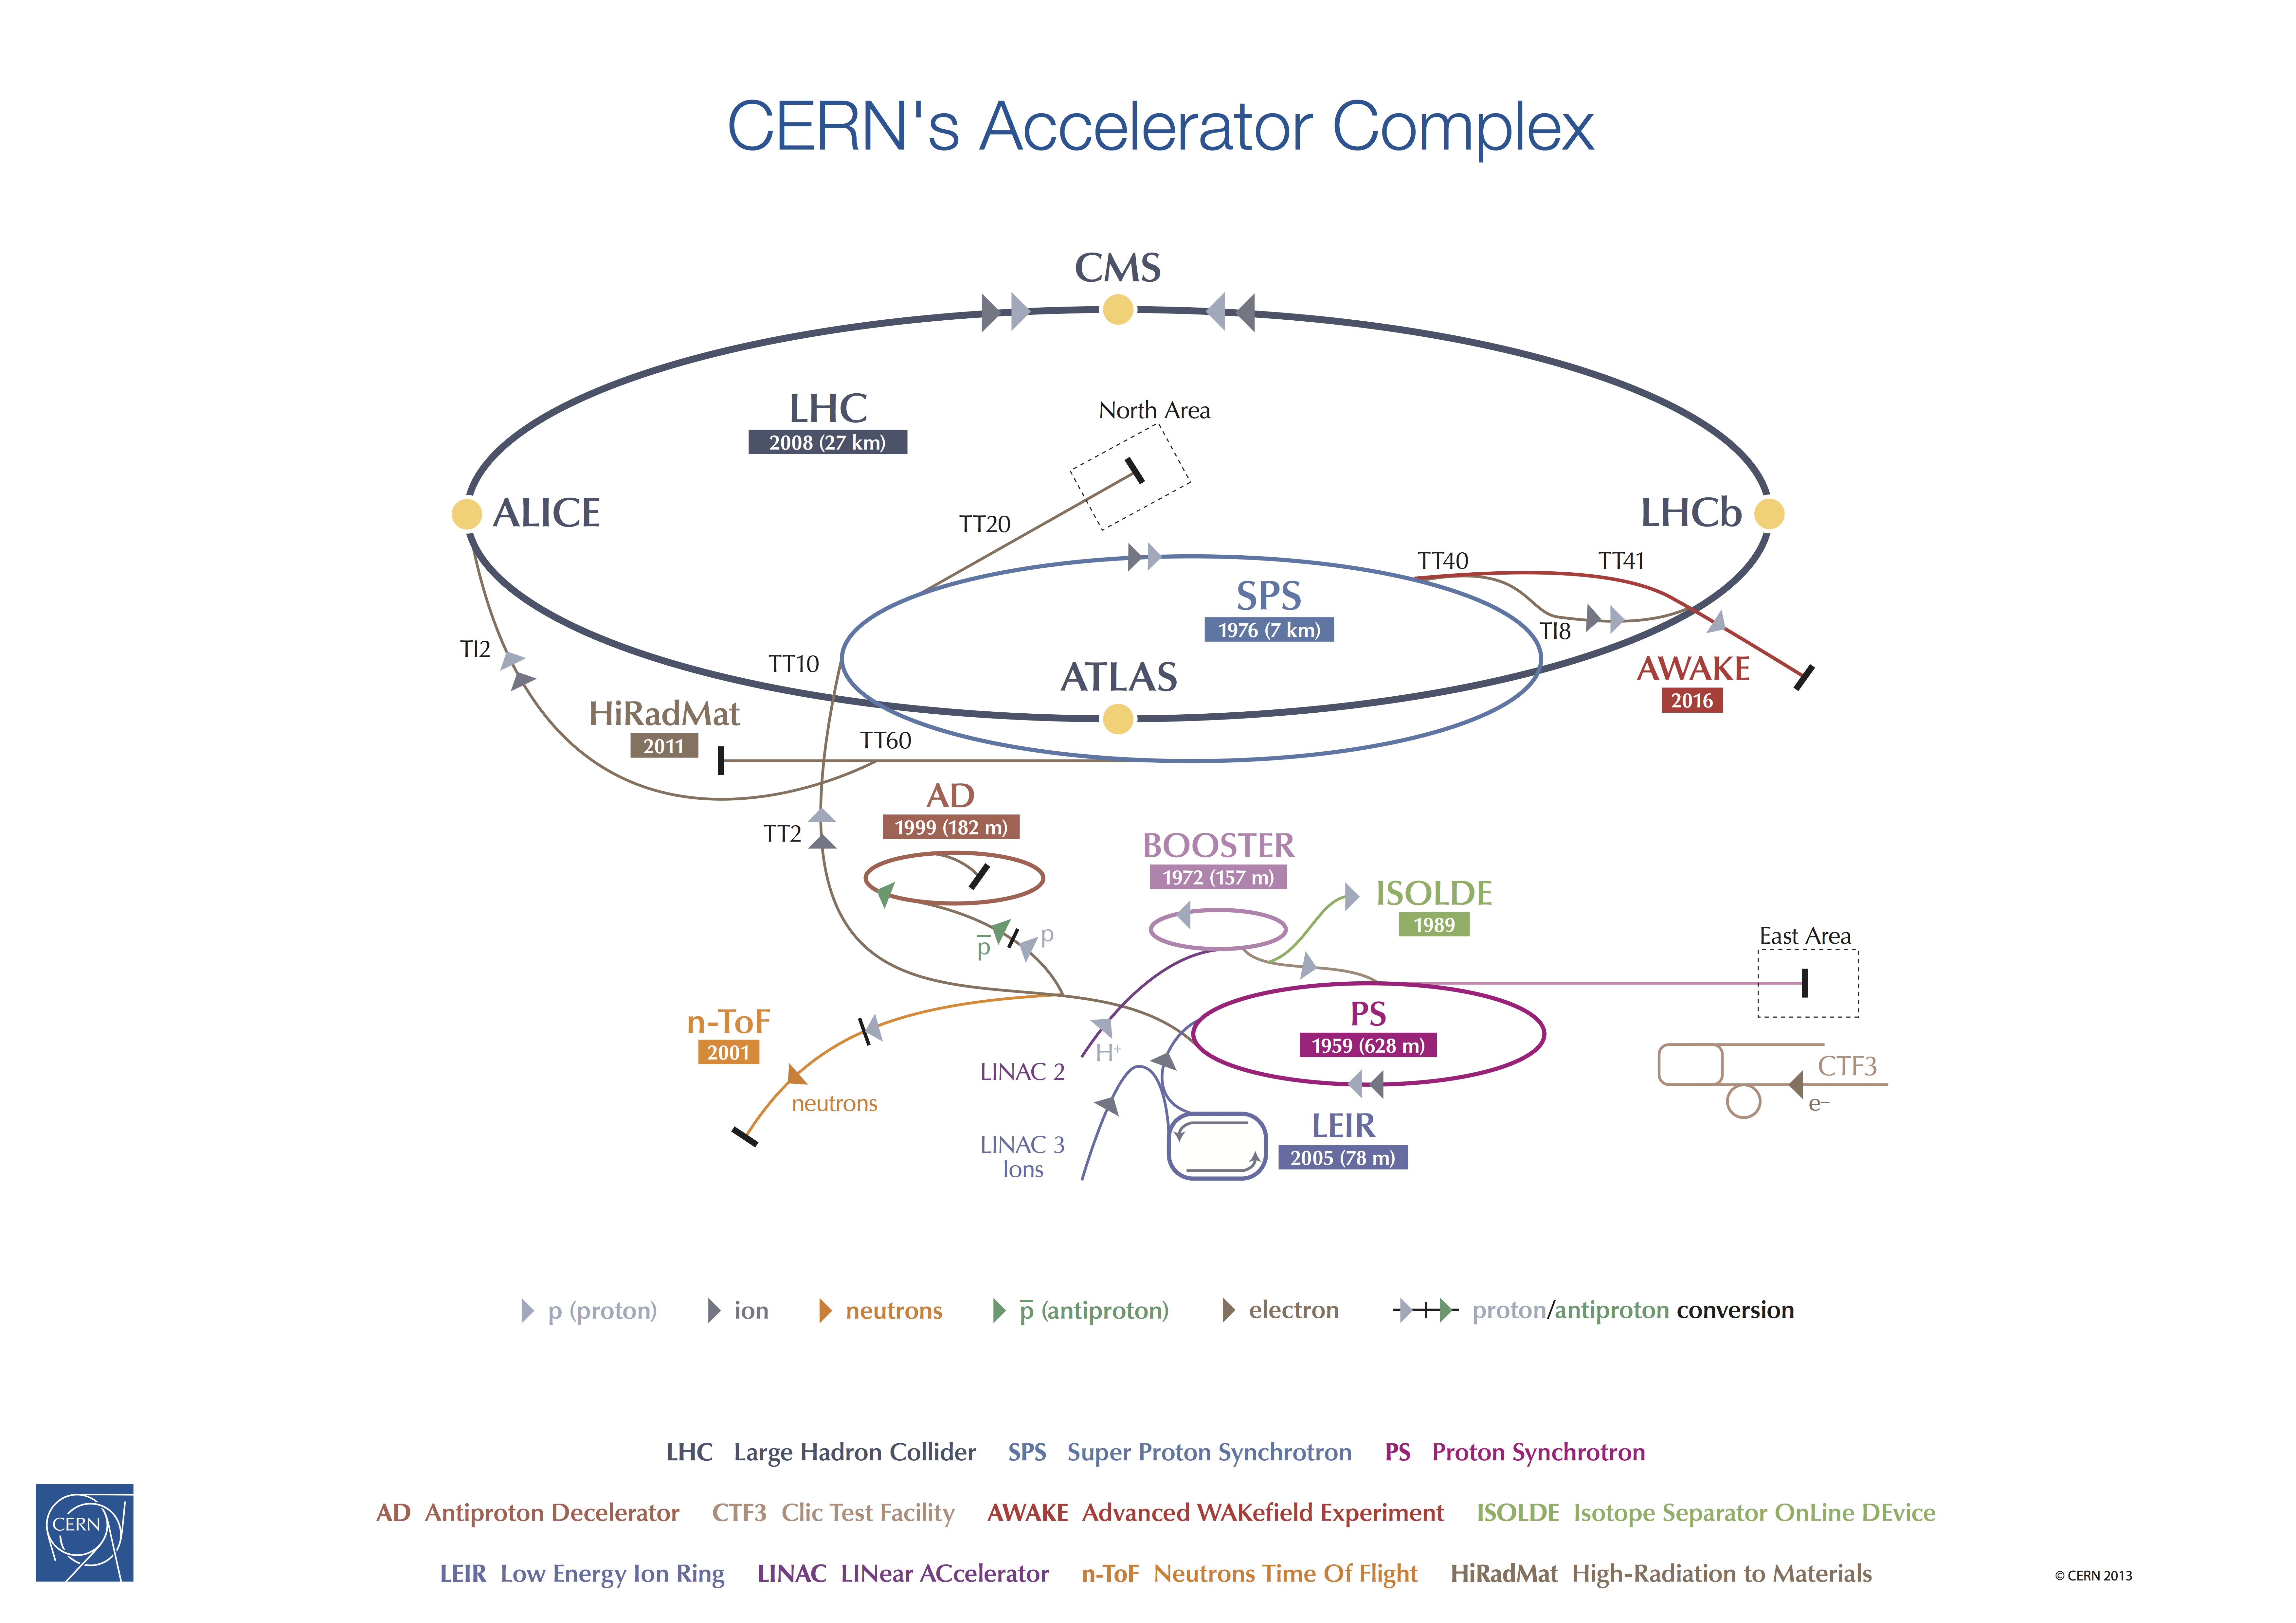
\includegraphics[width=0.9\linewidth]{figures/lhc/injection.jpg}
    \caption{ CERN accelerator complex} 
    \label{fig:injection_chain} 
  \end{center} 
\end{figure}

We begin with the most common element in the Universe, hydrogen, as our source
of protons.  A bottle of hydrogen gas provides 100 microsecond pulses of raw
$H_{2}$ which is then injected into a Duoplasmatron. There,  a strong electric
field and free elctrons from a cathode ionize the molecule into bare $H^{+}$
aka a proton!  These protons are then accelerated by a 90kV electric field,
leaving the Duoplasmatron at 1.4\% the speed of light ($\sim$4000km/s) or, in
Particle Physics units, about 83KeV. The bare protons are then fed into the
accelerating Radio Frequency (RF) cavities of Linear Accelerator 2 (LINAC2).
Inside, conductors charged by a powerful oscillating electromagnetic field
accelerate the protons to an energy of 50MeV. Along the way, small
quadrupole magnets shape the proton bunch ensuring they remain in a tight
beam.  This pattern of acceleration with RF cavities and shaping/tuning with
magnets is then repeated with CERN's first synchrotron, the Proton Synchrotron
(PS) rendering a 1.4 GeV proton beam.  The final step before the LHC comes with the
Super Proton Synchrotron where the same technologies are implemented to produce
450 GeV protons, ready for injection into the LHC. A diagrammatic representation
of this chain can be seen in \Cref{fig:injection_chain}. 

In order to produce proton-proton collisions, the LHC uses two beams
circulating in opposite directions.  The beams are not continuous, but instead
consist of bunches of $\mathcal{O}(10^{11})$ protons with a spacing of 25ns.
Given the LHC circumference this allows for 3564 bunches, however only 2808 are
filled per beam due to safety requirements and injection limitations.  Each
beam takes 4 minutes and 20 seconds to fill and then an additional 20 minutes
to for the protons to reach their maximum energy of 7 TeV, or 99.99999991\%
the speed of light! Under normal operating conditions these beams can be used
for many hours.

\section{LHC Layout and Design} \label{sec:lhc:layout}

While often depicted as a perfect circle the LHC is in reality an octagon with
rounded edges, called arcs, as can be seen in \Cref{fig:lhc_schematic}.
The counter-circulating beams of protons are depicted in red and
blue.  These beams are focused and collided at the 4 dedicated interaction
points at rates of up to 40 MHz.  Two of these points are occupied by the
ATLAS and CMS experiments, both of which are high luminosity, multi-purpose
experiments.

\begin{figure}[!htbp] 
  \begin{center}
    \includegraphics[width=0.9\linewidth]{figures/lhc/lhc_schematic.jpg}
    \caption{Labeled diagram of all the experiments at the LHC indicating the
counter-circulating beams and the relative location of each major experiment
along the circumference of the accelerator \cite{BATTISTONI:2011ujk}.} 
    \label{fig:lhc_schematic} 
  \end{center} 
\end{figure}

The exact design of the LHC tunnel is due to the experimental constraints of the
original machine for which it was built, the Large Electron Positron (LEP)
Collider.  For the $\sim 2,000$ times lighter electron the maximum energy was
limited by synchrotron radiation, proportional to $\frac{1}{m^4}$, requiring
long straight sections of accelerating RF cavities to recuperate the lost
energy.  Because this effect is $\mathcal{O}(10^{13})$ times smaller for the
proton, the LHC is instead limited by the ability to design and construct magnets
strong enough to bend the beam given the already determined curvature of the 8
arcs.

\begin{figure}[!htbp] 
  \begin{center}
    \includegraphics[width=0.9\linewidth]{figures/lhc/dipole.jpg}
    \caption{ Depiction of a LHC dipole magnet 2-in-1 design labeling the major
components \cite{Dailler:842530}.} 
    \label{fig:dipole} 
  \end{center} 
\end{figure}

The oppositely circulating beams must each have their own ring and magnetic field
which led to the creation of a twin-bore (i.e. ``two-in-one") magnet design, a
cross section of which can be seen in \Cref{fig:dipole}. These magnets are constructed
using NbTi superconductors which are cooled to 2 K using superfluid helium.
These magnets are design to provide the needed 8.33 T magnetic field required
to bend the proton trajectories at the designed beam energy of 7 TeV.  In total 1231 of these 15
m bending dipole magnets are used, in association with 392 5-7 m
quadrupole magnets which are responsible for keeping the proton bunches in a
tight beam by squeezing them both horizontally and vertically.

\section{Performance} \label{sec:lhc:performance}

Since the begining of its stable running in 2010 the LHC has performed well,
exceeding expectations.  While the LHC operation itself is incredibly complex,
the performance of the machine, for the purposes of analysis, can be reduced to
three numbers; the familiar center of mass energy of the beams, the integrated
luminosity and the instantaneous luminosity.  

For particle physics the integrated luminosity is proportional to the total
number of collisions recorded during a specified time period, while the
instantaneous luminosity is a function of the number of protons per bunch, the
bunch crossing rate and the cross section of a proton-proton interaction and
represents the particle flux.  Knowing this one can see that the integrated
luminosity, $L_{\text{int}}$ is simply the integral of the instantaneous luminosity
$L_{\text{inst.}}$ for a chosen data period as seen in
\Cref{eq:integrated_luminosity}.

\begin{equation} \label{eq:integrated_luminosity}
   L_{\text{int}} = \int L_{\text{inst.}}dt 
\end{equation}

For a standard Gaussian beam, $L_{\text{inst.}}$ can be written as

\begin{equation} \label{eq:inst_luminosity}
  L_{\text{inst.}} = \frac{N_{b}^{2}n_{b}f_{\text{rev}}\gamma_{r}}{4\pi\epsilon_{n}\beta^{*}}F
\end{equation}

where $N_{b}$ is the number of particles per bunch, $n_{b}$ the number of
bunches per beam, $f_{\text{rev}}$ the revolution frequency, $\gamma_{r}$ the
relativistic gamma factor, $\epsilon_{n}$ the normalized transverse beam
emittance, $\beta^{*}$ the beta function at the collision point, and $F$ the
geometric luminosity reduction factor due to the crossing angle at the
interaction point given by

\begin{equation}
  F = \bigg(1 + \Big( \frac{\theta_{c}\sigma_{z}}{2\sigma^{*}} \Big) ^{2}
\bigg)^{-1/2} 
\end{equation}

where $\theta_{c}$ is the full crossing angle at the interaction point,
$\sigma_{z}$ is the RMS bunch length, and $\sigma^{*}$ is the transverse RMS
beam size at the interaction point \cite{Evans:2008zzb}. Nominal values for the
above quantities are shown in \Cref{table:nominal_values} which also
demonstrates the incredible success of the LHC operators and accelerator teams
during the LHC Run II data taking period.

\begin{table}[htpb]
 \centering
 \caption{
  Nominal design values of LHC operations parameters at ATLAS for $25~\textrm{ns}$ bunch crossing spacing~\cite{Evans:2008zzb,PhysRevAccelBeams.19.101003}.
  Design and ATLAS recorded values of the machine luminosity are also given for LHC Run II operations~\cite{TWiki:2018ATLASPeakLumi}.
 }
 \begin{tabular}{@{}llr@{}} \toprule
  Parameter                                   & Symbol             & LHC Run II Value                \\ \midrule
  LHC circumference                           &                    & $26,659~\mathrm{m}$             \\
  LHC design beam energy                      &                    & $7~\TeV$                        \\
  LHC beam energy in Run II                   &                    & $6.5~\TeV$                      \\
  Number of protons per bunch                 & $N_{b}$            & $1.15 \times 10^{11}$           \\
  Number of proton bunches per beam           & $n_{b}$            & $2,808$                         \\
  Revolution frequency                        & $f_{\textrm{rev}}$ & $11.245~\mathrm{kHz}$           \\
  Lorentz factor (design)                     & $\gamma_{r}$       & $7462.69$                       \\
  Lorentz factor at $\sqrt{s} = 13~\TeV$      &                    & $6929.64$                       \\
  Normalized transverse beam emittance        & $\epsilon_{n}$     & $3.75~\mu\mathrm{m}$            \\
  Collision point beta function               & $\beta^{*}$        & $0.55~\mathrm{m}$               \\
  Full crossing angle                         & $\theta_{c}$       & $285~\mu\mathrm{rad}$           \\
  RMS bunch length                            & $\sigma_{z}$       & $7.55\times 10^{-2}~\mathrm{m}$ \\
  Transverse RMS beam size                    & $\sigma^{*}$       & $16.6~\mu\mathrm{m}$            \\ \midrule
  Peak design machine luminosity at $13~\TeV$ & $L_{\text{inst.}}$ & $9~\inb\mathrm{s}^{-1}$         \\
  Peak ATLAS recorded machine luminosity      &                    & $21~\inb\mathrm{s}^{-1}$        \\
  \bottomrule
 \end{tabular}\label{table:nominal_values}
\end{table}

The ATLAS experiment integrated luminosity for each year can be seen in
\Cref{fig:intlumivsyear} along with an example of the instantaneous luminosity
for $2017$ in \Cref{fig:peakLumiByFill} which is used in the presented analysis.

\begin{figure}[!htbp] 
\centering
\subcaptionbox{Integrated Luminosity 2011 - 2018\label{fig:intlumivsyear}}{\includegraphics[width=0.5\textwidth]{figures/lhc/intlumivsyear.pdf}}\hfill
\subcaptionbox{2017 Peak Instantaneous Luminosity\label{fig:peakLumiByFill}}{\includegraphics[width=0.5\textwidth]{figures/lhc/peakLumiByFill.pdf}}\hfill
\caption{Luminosity is monitored as both a running total known as the
integrated luminosity as depicted in (a) and as an instantaneous quantity as
shown in (b) \cite{LuminosityPublicResultsRun2}.}
\label{fig:luminosity} 
\end{figure}


\section{Pile-up at the LHC} \label{sec:lhc:pileup}

Given the large number of protons per bunch and the cross-section of a
proton-proton interaction, the probability to observe multiple interactions per
bunch crossing is quite high.  These multiple-interaction are known as pile-up,
$\mu$ or the time averaged representation $\langle \mu \rangle$, and come in two
different forms: 

\begin{enumerate} \item \textbf{In-time pile-up:} These are the other
proton-proton collisions that occur during the same bunch crossing as the
primary interaction that cauesd the Data Aquisition (DAQ) system to trigger.
These are the standard extra interactions we expect to observe as stated above.
\item \textbf{Out-of-time pile-up:} These are interactions that occur either
before or after a bunch crossing that causes the DAQ to trigger.  This effect is
generally due to the long integration times of some detector electronics.
\end{enumerate}

The pile-up profile for past years can be seen in figure XXX.  The width of this
distributino is due a combination of Poisonian statistics, the decrease in
number of protons per bunch over the lifetime of a single run, and optimization
tweaks to the beam's profile during runtime.  Understanding and eliminating the
noise from these pile-up events is crucial to reconstructing physics variables
to represent the primary interaction we hope to observe.


\chapter{The ATLAS Detector} \label{chap:atlas}

Given the immense energies availalbe at the LHC, and the veritable zoo of
paricles we are trying to detect, we require a general-purpose experiment in
order to fully exploit the full range of physics opportunities provided.  Two
international collaborations rose to this challenge, the CMS (Compact Muon
Solenoid) and ATLAS (A Torroidal LHC ApparatuS) experiments.  While both have
similar physics goals and each of them strengths and weaknesses, this
dissertation will focus on the ATLAS experiment and the intricacies of its three
main sub-detectors and two massive magnet systems.  

Located approximately 100 meters underground in a vast excavated chamber, the
ATLAS detector rests its 7000 metric tonnes on a bed of concrete reinforced
steel.  Out of it flows the signals of over 100 million electronic channels
through a zip tied mass of greater than 3000 kilometers of cabling.  At its very
center is one of the four interaction points of the LHC, specifically Point 1,
where the two counter circulating proton beams are skillfully shaped and then
collided by a series of magnets.  The energetic particles resultant from this
collision then fly out in all directions into the bulk of the ATLAS detector.

The first sub-system they meet is the Inner Detector (ID) and its many layers of
strip and pixel silcon detectors along with a transition radiation gaseous wire
detector, all bathed in the 2T mangnetic field of the surronding superconducting
solenoidal magnet.  This system exploits the ionization of charged particles to
track their curved trajectory through the magnetic field.  This curvature gives
us charge information, a momentum measurement, and precision 3D verticies
crucial to the identification of the secondary verticies of a b-hadron decay. 

Outside of the solenoid the particles are faced with first the Electromagnetic
and then the Hadronic sampling calorimeters. Here, layers of scintillator and 
high radiation length materials are implemented to measure the energy of
electrons, photons, and hadrons.  The goal being to absorb all of the energy of
the partilces in order to have an accurate measurement.

Finally we have the muon system surrounding the calorimeter and equipped with
its own torroidal magnet system.  Here the charged muon bends in the magnetic
field while leaving a trail of ionization in the muon spectrometer before
exiting the detector completely.  Neutrinos are the only other standard model
particle that leave the detector, however they do so without detection.

In the following sections I will explain our choosen coordinate system and give 
a more detailed reveiw of these 3 detector sub-systems.  

\section{ATLAS Coordinate System} \label{sec:atlas:coordinates}

Using the nominal interaction point as the origin, ATLAS uses a right-handed
coordinate system where the positive $x$-axis points towards the center of the
LHC ring, the positive $y$-axis points upwards, and the positive $z$-axis is
defined by the counter clockwise circulating beam direction as viewed from
above shown in \Cref{fig:atlas_geometry} \cite{PERF-2007-01}.  
 
\begin{figure}[!htbp]
  \begin{center}
    \includegraphics[width=0.5\linewidth]{figures/atlas/atlas_geometry}
    \caption{ \cite{Stark:2317296} A cartoon view of the the LHC from above
showing the SPS, LHC and the four main experiments of the LHC: ATLAS, CMS, LHCb,
and ALICE.  The standard cartesian coordinate system is shown with its origin at
the ATLAS interaction point, the positive $x$-axis towards the center of the
LHC, the positive $y$-axis pointing upwards, and the positive $z$-axis pointing
along the beamline towards the "A-side"}
    \label{fig:atlas_geometry}
  \end{center}
\end{figure}

Using these coordinates we can define the physical momentum of the objects
measured as $\vec{p} = (\pt,p_z)$ with \pt being the momentum of the object in
the transverse plane and $p_z$ the momentum along the beam axis. Given the
cylindrical symmetry of ATLAS it is desirable to define the polar angle
$\theta$ from the beam axis with the $r$-$\phi$ plane being perpendicular to that
axis. Since the particles we observe are relativistically boosted in the
$z$-axis it is desirable to use the Lorentz invariant quantity pseudorapidity
$(\eta)$ defined in terms of the polar angle by

\begin{equation}
 \eta = -\ln \tan \left( \frac{\theta}{2} \right).
\end{equation}

where $\eta = 0$ is in the $x$-$y$ plane and larger values of $|\eta|$ being
closer to the beam axis as can be seen in \Cref{fig:pseudorapidity}.

\begin{figure}[!htbp]
  \begin{center}
    \includegraphics[width=0.5\linewidth]{figures/atlas/pseudorapidity}
    \caption{Modified from \cite{Stark:2317296} this cartoon represents a
selection of pseudorapiditity $(\eta)$ values overlaid with some cartesian
coordinates (dashed black lines).  The red lines are drawn for $\eta = \pm
0.5,1.0,3.0$ }
    \label{fig:pseudorapidity}
  \end{center}
\end{figure}

In this analysis the angular separation between objects in the detector is
calculated and represented using the geometric quantity 

\begin{equation}
 \DeltaRdef
\end{equation}
 
\section{Tracking with the Inner Detector} \label{sec:atlas:tracking}

With its closest component, the insertable b-layer (IBL)
\cite{Potamianos:2209070}, only 3.3 cm from the beampipe The Inner Detector
(ID), shown in figure \ref{fig:inner_detector_diagram}
\cite{ATLAS-TDR-4,ATLAS-TDR-5} faces the incredible challenge of providing
precision momentum resolution and identification of both primary and secondary
vertex measurements of charged tracks all while recieving the highest fluence of any detector.

\begin{figure}[!htbp]
  \begin{center}
    \includegraphics[width=0.8\linewidth]{figures/atlas/inner_detector_diagram}
    \caption{ \cite{Potamianos:2209070} Diagram of inner detector}
    \label{fig:inner_detector_diagram}
  \end{center}
\end{figure}

It is designed to be very compact to fit inside the 2T solenoid and to give
excellent momentum resolution above the nominal \pT threshold of $0.5$GeV and
within the pseudorapidity range of $|\eta| < 2.5$ as shown in figure \ref{fig:inner_detector_schematic}

\begin{figure}[!htbp]
  \begin{center}
    \includegraphics[width=0.8\linewidth]{figures/atlas/inner_detector_schematic}
    \caption{ \cite{PIX-2018-001} Schematic of the Inner Detector including eta lines}
    \label{fig:inner_detector_schematic}
  \end{center}
\end{figure}

 
\section{Calorimetry} \label{sec:atlas:calorimetry}

\section{Muon Spectrometer} \label{sec:atlas:muons}

The ATLAS Muon Spectrometer (MS) \cite{PERF-2007-01}, see figure
\ref{fig:muon_system}, accomplishes tracking of charged particles in the $|\eta|
< 2.7$ region for momentum reconstruction while also providing triggering on
charged particles in the $|\eta| < 2.4$ region.  The magnetic field necessary
for momentum reconstruction is provided by 3 air core torroid systems, one
barrel torrioid covering $|\eta| < 1.4$ and two endcap torroid systems which are
inserted into the inner radius of the the barrel torroid to cover the $1.6 <
|\eta| < 2.7$. The so called transition region $1.4 < |\eta| < 1.6$ between
these two magnet systems is covered by a combination of the barrel and endcap
torroid magnets.  Similar to the ID the resolution is inversely proportional to
the particle's incident momentum.  Any muon with pT lower than ~3GeV will never
make it to the MS and thus will not be detected.  

\begin{figure}[!htbp]
  \begin{center}
    \includegraphics[width=0.8\linewidth]{figures/atlas/muon_system}
    \caption{ \cite{PERF-2007-01} A cut-away diagram of the ATLAS muon system
and its many sub-detectors.}
    \label{fig:muon_system}
  \end{center}
\end{figure}

Precision tracking measurements for momentum reconstruction is accomplished
using the Monitored Drift Tube chambers (MDTs) for $|\eta| < 2.0$ and using
Cathode-Strip Chambers (CSCs) for $2.0 < |\eta| < 2.7$.  The MDT system consists of
1163 drift tube chambers arranged in three to eight layers for varying $\eta$.
The CSCs are designed to withstand the higher rate and retain good time
resolution using multiwire proportional chambers with orthogonal segmented
cathode planes.

The MS also gives nanosecond tracking information for triggering on muon tracks.
This is accomplished using Resistive Plate Chambers (RPC) in the barrel region
$|\eta| < 1.05$ and Thin Gap Chambers (TGC) in the end-cap $1.05 < |\eta| < 2.4$
region.  Both chamber systems deliver a triggerable signal with a spread of
$15-25$ ns, thus providing the ability to tag individual beam-crossings.



\part{The HbbISR Analysis}
% The analysis 

\chapter{Data and Monte-Carlo Simulation} \label{chap:data}

This analysis focuses on the data collected by the ATLAS detector from \pp
collisions produced by the LHC at the center-of-mass-energy of 13 TeV.  In
particular the analysis shown uses datasets collected in 2015, 2016, and 2017
and ammounts to an integrated luminosity of $80.5 \text{ fb}^{-1}$ after beam,
detector and data-quality requirements are taken into account. 

In order to compare our findings with theory, we use the predictions of the SM
to produce Monte-Carlo (MC) simulated events to model the signal and background
processes.  These MC samples go through a full simulation of the ATLAS detector
and are reconstructed using the same algorithms as used on data such that the
MC and Data have the same format at analysis level. This allows us to analyze
the MC and Data using the same framework such that we can make direct
comparisons between theory and reality as our final product.

The following sections discuss the systems for selecting the data used in the
analysis as well as the software packages, developed in collaboration with
theorists, used to simulate the signal and background processes of the
analysis.

\section{Data Used} \label{sec:data:data}

As mentioned before the data used is checked to make sure it is of high
quality, meaning that the beam, detector and data collection systems were all
fully opperational during the event in question. These data quality
requirements are enfored by choosing only events from each respective years
Good Runs List (GRL), an XML file produced by the ATLAS data quality
monitoring team that lists all events that have met the data quality critera.
This analysis uses three such GRLs - one for each year of data taking
(2015,2016,2017) - corresponding to annual integrated luminosities of $3.2
\text{ fb}^{-1}$, $33 \text{ fb}^{-1}$, and $44.3 \text{ fb}^{-1}$.

\section{Higgs Boson Signal Monte Carlo Samples} \label{sec:data:signal_mc}

In order to simulate Higgs boson events, the three leading production
mechanisms at the LHC were considered, shown in \Cref{fig:higgs_production}:
gluon-gluon fusion, vector boson fusion and Higgsstrahlung.  These three
production modes represent approximately 88\%, 7\% and 4\% of the total Higgs
signal, respectively, before analysis cuts are applied.  In all samples the
simulated Higgs boson is forced to decay to the $b\bar{b}$ final state.
 
The ggF $H$ + jet events were generated using the HJ+MiNLO~\cite{Hamilton2015}
prescription, assuming a finite top quark mass, with the \textsc{Powheg-Box} 2
generator~\cite{Campbell2012} and the NNPDF30 NNLO parton distribution
functions~\cite{Hamilton:2012rf}.  After generation the events were showered
using \textsc{Pythia} 8.212~\cite{Sjostrand:2014zea} with the AZNLO tune and
the CTEQ6L1 parton distribution functions~\cite{Pumplin:2002vw}. Any
$b$-hadrons produced during this process were decayed using
\textsc{EvtGen}~\cite{LANGE2001152}. During generation a parton level filter of
$k_{T} > 200~\GeV$ was used to select high momentum events.  This filtering is
reflected in the cross section in \Cref{table:data:signal}.

The VBF $H$ + jet events were also generated using the \textsc{Powheg-Box}
generator~\cite{Nason:2009ai} with the NNPDF30 NLO parton distribution
functions~\cite{Hamilton:2012rf}. Again the showering was performed with
\textsc{Pythia} 8.212~\cite{Sjostrand:2014zea} using the AZNLO tune and the
CTEQ6L1 parton distribution functions~\cite{Pumplin:2002vw}.  The decay of
$b$-hadrons was again performed using \textsc{EvtGen}~\cite{LANGE2001152}.
During generation the produced Higgs boson was required to have a $p_{T} >
250~\GeV$.  This filtering is reflected in the filtering efficiency in
\Cref{table:data:signal}.

Higgsstrahlung events were generated using the \textsc{Pythia} 8.212
generator~\cite{Sjostrand:2014zea}, the AZNLO tune and the CTEQ6L1 parton
distribution functions~\cite{Pumplin:2002vw}.  Again the decay of $b$-hadrons
is handled by \textsc{EvtGen}~\cite{LANGE2001152}. Unfortunately the
\textsc{Pythia} $ZH$ process does not include the $gg \rightarrow ZH$
contribution.  To account for this the cross section is corrected to the LHC
Higgs cross section working group's (LHCHXSWG) recommended
$\sigma_{\text{NLO+NLL}}^{\text{ggZH}}$ with NLO + Next to Leading Log (NLL)
accuracy \cite{MelladoGarcia:2150771}. During generation a filter of $p_{T} >
350~\GeV$ was used to select for high momentum events. This
filtering is reflected in the filtering efficiency in \Cref{table:data:signal}.

\begin{sidewaystable}
  \centerline{
  \centering
  {\tiny
  \begin{tabular}{l|c|cccc}
    \textbf{Dataset} & \textbf{Campaign} & \textbf{xsec (pb)} & \shortstack{\textbf{Filter} \\ \textbf{Efficiency}} & \shortstack{\textbf{Events} \\ \textbf{Generated}} & \shortstack{\textbf{Effective} \\  \textbf{Luminosity (\ifb)}} \\
    \hline
    \hline
    309450.PowhegPy8EG\_NNLOPS\_nnlo\_30\_ggH125\_bb\_kt200 & MC16a & 0.4763 & 1.0 & 400000 & 839.1 \\
    345931.PowhegPy8EG\_NNPDF30\_AZNLOCTEQ6L1\_VBFH125\_bb & MC16a & 3.7296 & 0.026877 & 499500 & 4794 \\
    309451.Pythia8EvtGen\_A14NNPDF23LO\_WH125\_bb\_fj350 & MC16a & 0.63487 & 0.01306 & 100000 & 12061 \\
    309452.Pythia8EvtGen\_A14NNPDF23LO\_ZH125\_bb\_fj350 & MC16a & 0.34656 & 0.013036 & 100000 & 22135 \\
    \hline
    309450.PowhegPy8EG\_NNLOPS\_nnlo\_30\_ggH125\_bb\_kt200 & MC16d & 0.4763 & 1.0 & 499000 & 1047 \\
    345931.PowhegPy8EG\_NNPDF30\_AZNLOCTEQ6L1\_VBFH125\_bb & MC16d & 3.7296 & 0.026877 & 650000 & 6238 \\
    309451.Pythia8EvtGen\_A14NNPDF23LO\_WH125\_bb\_fj350 & MC16d & 0.63487 & 0.01306 & 130000 & 15679 \\
    309452.Pythia8EvtGen\_A14NNPDF23LO\_ZH125\_bb\_fj350 & MC16d & 0.34656 & 0.013036 & 130000 & 28775 \\
  \end{tabular}}
  }
\caption{List of datasets used for Higgs boson Monte Carlo \cite{Krizka:2310645}.}
\label{table:data:signal}
\end{sidewaystable}



\section{Background Monte Carlo} \label{sec:data:bkg_mc}

Modeling the expected contributions of backgrounds to the analysis is done with
a mix of data driven methods and Monte Carlo simulated samples as discussed in
\Cref{chap:background}.  The MC samples were used for the development of the
modeling of the non-resonant QCD multijet backgrounds and for the estimation
of the major resonant backgrounds from $V$+jet, $t\bar{t}$, and single-top
production.  For the multijet background the final estimation is data driven,
but the MC was used to develop the background model.

The QCD dijet events were simulated by the \textsc{Pythia} 8.186
generator~\cite{Sjostrand:2007gs} with the A14 tune and the NNPDF23 LO
PDF~\cite{Carrazza:2013axa} using \textsc{EvtGen} to decay the resulting
$b$-hadrons~\cite{LANGE2001152}.  To maintain a constant statistical precision
over a large momentum range, the weighted events were generated with a flat \pT
spectrum. The QCD samples used to develop the background model are summarized
in \Cref{table:data:QCD}.

\begin{sidewaystable}
  \centerline{
  \centering
  {\tiny
  \begin{tabular}{l|c|cccc}
    \textbf{Dataset} & \textbf{Campaign} & \textbf{xsec (pb)} & \shortstack{\textbf{Filter} \\ \textbf{Efficiency}} & \shortstack{\textbf{Events} \\ \textbf{Generated}} & \shortstack{\textbf{Effective} \\  \textbf{Luminosity (\ifb)}} \\
    \hline
    \hline
    361020.Pythia8EvtGen\_A14NNPDF23LO\_jetjet\_JZ0W & MC16a & 78420e+06 & 0.9755 & 16000000 & 2.0915e-07 \\
    361021.Pythia8EvtGen\_A14NNPDF23LO\_jetjet\_JZ1W & MC16a & 78420e+06 & 0.00067143 & 15998000 & 7.5762e-05 \\
    361022.Pythia8EvtGen\_A14NNPDF23LO\_jetjet\_JZ2W & MC16a & 24332e+05 & 0.00033423 & 15989500 & 0.0053309 \\
    361023.Pythia8EvtGen\_A14NNPDF23LO\_jetjet\_JZ3W & MC16a & 26454e+03 & 0.00032016 & 15879500 & 0.44989 \\
    361024.Pythia8EvtGen\_A14NNPDF23LO\_jetjet\_JZ4W & MC16a & 25463e+01 & 0.00053138 & 15925500 & 29.858 \\
    361025.Pythia8EvtGen\_A14NNPDF23LO\_jetjet\_JZ5W & MC16a & 4553.5 & 0.00092409 & 15993500 & 1103.2 \\
    361026.Pythia8EvtGen\_A14NNPDF23LO\_jetjet\_JZ6W & MC16a & 257.53 & 0.00094242 & 17834000 & 25916 \\
    361027.Pythia8EvtGen\_A14NNPDF23LO\_jetjet\_JZ7W & MC16a & 16.215 & 0.0003928 & 15983000 & 35888 \\
    361028.Pythia8EvtGen\_A14NNPDF23LO\_jetjet\_JZ8W & MC16a & 0.62503 & 0.010176 & 15999000 & 25154e+02 \\
    361029.Pythia8EvtGen\_A14NNPDF23LO\_jetjet\_JZ9W & MC16a & 0.019639 & 0.012076 & 13995500 & 59013e+03 \\
    361030.Pythia8EvtGen\_A14NNPDF23LO\_jetjet\_JZ10W & MC16a & 0.0011962 & 0.0059087 & 13985000 & 19786e+05 \\
    361031.Pythia8EvtGen\_A14NNPDF23LO\_jetjet\_JZ11W & MC16a & 4.2259e-05 & 0.0026761 & 15948000 & 1.4102e+11 \\
    361032.Pythia8EvtGen\_A14NNPDF23LO\_jetjet\_JZ12W & MC16a & 1.0367e-06 & 0.00042592 & 15995600 & 3.6226e+13 \\
    \hline
    361020.Pythia8EvtGen\_A14NNPDF23LO\_jetjet\_JZ0W & MC16d & 78420e+06 & 0.9755 & 15987000 & 2.0898e-07 \\
    361021.Pythia8EvtGen\_A14NNPDF23LO\_jetjet\_JZ1W & MC16d & 78420e+06 & 0.00067143 & 15997000 & 7.5728e-05 \\
    361022.Pythia8EvtGen\_A14NNPDF23LO\_jetjet\_JZ2W & MC16d & 24332e+05 & 0.00033423 & 15981000 & 0.005331 \\
    361023.Pythia8EvtGen\_A14NNPDF23LO\_jetjet\_JZ3W & MC16d & 26454e+03 & 0.00032016 & 15878500 & 0.45043 \\
    361024.Pythia8EvtGen\_A14NNPDF23LO\_jetjet\_JZ4W & MC16d & 25463e+01 & 0.00053138 & 15974500 & 29.968 \\
    361025.Pythia8EvtGen\_A14NNPDF23LO\_jetjet\_JZ5W & MC16d & 4553.5 & 0.00092409 & 15991500 & 1103.6 \\
    361026.Pythia8EvtGen\_A14NNPDF23LO\_jetjet\_JZ6W & MC16d & 257.53 & 0.00094242 & 17880400 & 25979 \\
    361027.Pythia8EvtGen\_A14NNPDF23LO\_jetjet\_JZ7W & MC16d & 16.215 & 0.0003928 & 15116500 & 33886e+01 \\
    361028.Pythia8EvtGen\_A14NNPDF23LO\_jetjet\_JZ8W & MC16d & 0.62503 & 0.010176 & 15987000 & 25136e+02 \\
    361029.Pythia8EvtGen\_A14NNPDF23LO\_jetjet\_JZ9W & MC16d & 0.019639 & 0.012076 & 14511500 & 61189+03 \\
    361030.Pythia8EvtGen\_A14NNPDF23LO\_jetjet\_JZ10W & MC16d & 0.0011962 & 0.0059087 & 15988000 & 22620e+05 \\
    361031.Pythia8EvtGen\_A14NNPDF23LO\_jetjet\_JZ11W & MC16d & 4.2259e-05 & 0.0026761 & 15993000 & 1.4142e+11 \\
    361032.Pythia8EvtGen\_A14NNPDF23LO\_jetjet\_JZ12W & MC16d & 1.0367e-06 & 0.00042592 & 15640000 & 3.5421e+13 \\
  \end{tabular}}
  }
\caption{List of datasets used for QCD Monte Carlo \cite{Krizka:2310645}.}
\label{table:data:QCD}
\end{sidewaystable}

Hadronically decaying $W$ and $Z$ events were produced with a maximum of four
additional partons at leading order (LO).  This was accomplished with the
\textsc{Sherpa} 2.1.1 generator~\cite{Gleisberg:2008ta} and the CT10 parton
distribution functions~\cite{Lai:2010vv}.  For leptonically decaying $W$ and
$Z$ events samples were produced with a maximum of two additional partons at LO
and a maximum of two at next-to-leading order (NLO).  Next the LO hadronic $W$
and $Z$ cross sections were corrected by applying multiplicative ``$k$-factors"
derived from the corresponding NLO leptonic $W$ and $Z$ samples.  These
corrections were 1.28 for the $W$+jets and 1.37 for the $Z$+jets
\cite{Aaboud:2018zba}. An alternate sample of hadronically decaying $W$ and $Z$
events was produced for cross checks using the \text{Herwig}++2.7.1
generator~\cite{Bahr:2008pv} with the UEEE4 tune~\cite{Buckley:2018wdv} and the
CTEQ6L1~\cite{Pumplin:2002vw}.  Unlike the \textsc{Sherpa} samples these
\textsc{Herwig} samples only contained one additional parton in the matrix
element. The hadronic $W$+jets and $Z$+jets samples used in this
analysis~\footnote{Note that the leptonically decaying $W$ and $Z$
samples were only used to derive correction factors and thus are not
presented.} are summarized in \Cref{table:data:V_hadronic}.

\begin{sidewaystable}
  \centerline{
  \centering
  {\tiny
  \begin{tabular}{l|c|cccc}
    \textbf{Dataset} & \textbf{Campaign} & \textbf{xsec (pb)} & \shortstack{\textbf{Filter} \\ \textbf{Efficiency}} & \shortstack{\textbf{Events} \\ \textbf{Generated}} & \shortstack{\textbf{Effective} \\  \textbf{Luminosity (\ifb)}} \\
    \hline
    \hline
    304307.Sherpa\_CT10\_Wqq\_Pt280\_500 & MC16a & 29.487 & 1.0 & 150000 & 4.8429 \\
    304308.Sherpa\_CT10\_Wqq\_Pt500\_1000 & MC16a & 2.162 & 1.0 & 30000 & 12.646 \\
    304309.Sherpa\_CT10\_Wqq\_Pt1000 & MC16a & 0.046218 & 1.0 & 15000 & 273.61 \\
    \hline
    304307.Sherpa\_CT10\_Wqq\_Pt280\_500 & MC16d & 29.481 & 1.0 & 140000 & 4.5533 \\
    304308.Sherpa\_CT10\_Wqq\_Pt500\_1000 & MC16d & 2.1642 & 1.0 & 30000 & 13.431 \\
    304309.Sherpa\_CT10\_Wqq\_Pt1000 & MC16d & 0.046152 & 1.0 & 15000 & 287.55 \\
    \hline
    \hline
    304707.Sherpa\_CT10\_Zqq\_Pt280\_500 & MC16a & 12.623 & 1.0 & 75000 & 5.8079 \\
    304708.Sherpa\_CT10\_Zqq\_Pt500\_1000 & MC16a & 0.90771 & 1.0 & 15000 & 16.090 \\
    304709.Sherpa\_CT10\_Zqq\_Pt1000 & MC16a & 0.018344 & 1.0 & 10000 & 251.86 \\
    \hline
    304707.Sherpa\_CT10\_Zqq\_Pt280\_500 & MC16d & 12.644 & 1.0 & 75000 & 5.6273 \\
    304708.Sherpa\_CT10\_Zqq\_Pt500\_1000 & MC16d & 0.90886 & 1.0 & 15000 & 16.278 \\
    304709.Sherpa\_CT10\_Zqq\_Pt1000 & MC16d & 0.018264 & 1.0 & 10000 & 524.45 \\
    \hline
    \hline
    304673.Herwigpp\_UEEE5CTEQ6L1\_Wjhadronic\_280\_500 & MC16a & 13.491 & 1.0 & 150000 & 11.119 \\
    304674.Herwigpp\_UEEE5CTEQ6L1\_Wjhadronic\_500\_700 & MC16a & 0.91592 & 1.0 & 39000 & 42.580 \\
    304675.Herwigpp\_UEEE5CTEQ6L1\_Wjhadronic\_700\_1000 & MC16a & 0.17413 & 1.0 & 30000 & 172.29 \\
    304676.Herwigpp\_UEEE5CTEQ6L1\_Wjhadronic\_1000\_1400 & MC16a & 0.021936 & 1.0 & 30000 & 1367.6 \\
    304677.Herwigpp\_UEEE5CTEQ6L1\_Wjhadronic\_1400 & MC16a & 0.0022502 & 1.0 & 20000 & 8888.1 \\
    \hline
    304673.Herwigpp\_UEEE5CTEQ6L1\_Wjhadronic\_280\_500 & MC16d & 13.491 & 1.0 & 190000 & 14.083 \\
    304674.Herwigpp\_UEEE5CTEQ6L1\_Wjhadronic\_500\_700 & MC16d & 0.91592 & 1.0 & 50000 & 54.590 \\
    304675.Herwigpp\_UEEE5CTEQ6L1\_Wjhadronic\_700\_1000 & MC16d & 0.17413 & 1.0 & 40000 & 229.71 \\
    304676.Herwigpp\_UEEE5CTEQ6L1\_Wjhadronic\_1000\_1400 & MC16d & 0.021936 & 1.0 & 40000 & 1823.5 \\
    304677.Herwigpp\_UEEE5CTEQ6L1\_Wjhadronic\_1400 & MC16d & 0.0022502 & 1.0 & 30000 & 13332 \\
    \hline
    \hline
    304678.Herwigpp\_UEEE5CTEQ6L1\_Zjhadronic\_280\_500 & MC16a & 5.4672 & 1.0 & 75000 & 13.718 \\
    304679.Herwigpp\_UEEE5CTEQ6L1\_Zjhadronic\_500\_700 & MC16a & 0.37032 & 1.0 & 20000 & 54.007 \\
    304680.Herwigpp\_UEEE5CTEQ6L1\_Zjhadronic\_700\_1000 & MC16a & 0.070961 & 1.0 & 15000 & 211.38 \\
    304681.Herwigpp\_UEEE5CTEQ6L1\_Zjhadronic\_1000\_1400 & MC16a & 0.0087931 & 1.0 & 15000 & 1705.9 \\
    304682.Herwigpp\_UEEE5CTEQ6L1\_Zjhadronic\_1400 & MC16a & 0.00089549 & 1.0 & 10000 & 11167 \\
    \hline
    304678.Herwigpp\_UEEE5CTEQ6L1\_Zjhadronic\_280\_500 & MC16d & 5.4672 & 1.0 & 100000 & 18.291 \\
    304679.Herwigpp\_UEEE5CTEQ6L1\_Zjhadronic\_500\_700 & MC16d & 0.37032 & 1.0 & 30000 & 81.011 \\
    304680.Herwigpp\_UEEE5CTEQ6L1\_Zjhadronic\_700\_1000 & MC16d & 0.070961 & 1.0 & 20000 & 281.84 \\
    304681.Herwigpp\_UEEE5CTEQ6L1\_Zjhadronic\_1000\_1400 & MC16d & 0.0087931 & 1.0 & 20000 & 2274.5 \\
    304682.Herwigpp\_UEEE5CTEQ6L1\_Zjhadronic\_1400 & MC16d & 0.00089549 & 1.0 & 20000 & 22334 \\
  \end{tabular}}
  }
\caption{List of datasets used for hadronically decaying $W$+jets and $Z$+jets Monte Carlo \cite{Krizka:2310645}.}
\label{table:data:V_hadronic}
\end{sidewaystable}

Our $t\bar{t}$ samples were generated using \textsc{Powheg-Box}
2~\cite{Campbell2012} and the NNPDF30 NLO parton distribution
functions~\cite{Ball:2014uwa}. After generation the events were showered using
\textsc{Pythia} 8.230~\cite{Sjostrand:2014zea} using the A14 tune and the
NNPDF23 LO parton distribution functions~\cite{Carrazza:2013axa} with all
$b$-hadron decays performed by \textsc{EvtGen}~\cite{LANGE2001152}.  The
samples were then broken up according to the decay mode of the two top quarks
into three categories; all-hadronic, semi-leptonic, all-leptonic. Additional
$t\bar{t}$ events were generated with the \textsc{Sherpa} 2.2.1
generator~\cite{Gleisberg:2008ta} using the NNPDF30 NNLO parton distribution
functions~\cite{Ball:2014uwa}.  This second sample was used as a cross check of
the main samples generated with \textsc{Powheg-Box} 2 + \textsc{Pythia} 8. The
$t\bar{t}$ samples used in this analysis are summarized in
\Cref{table:data:ttbar}.

\begin{sidewaystable}
  \centerline{
  \centering
  {\tiny
  \begin{tabular}{l|c|cccc}
    \textbf{Dataset} & \textbf{Campaign} & \textbf{xsec (pb)} & \shortstack{\textbf{Filter} \\ \textbf{Efficiency}} & \shortstack{\textbf{Events} \\ \textbf{Generated}} & \shortstack{\textbf{Effective} \\  \textbf{Luminosity (\ifb)}} \\
    \hline
    \hline
    410470.PhPy8EG\_A14\_ttbar\_hdamp258p75\_nonallhad & MC16a & 729.77 & 0.54384 & 60413000 & 148.78 \\
    410471.PhPy8EG\_A14\_ttbar\_hdamp258p75\_allhad & MC16a & 729.78 & 0.45627 & 19994000 & 59.101 \\
    410472.PhPy8EG\_A14\_ttbar\_hdamp258p75\_dil & MC16a & 729.77 & 0.10546 & 39974000 & 511.18 \\
    \hline
    410470.PhPy8EG\_A14\_ttbar\_hdamp258p75\_nonallhad & MC16d & 729.77 & 0.54384 & 74486000 & 184.71 \\
    410471.PhPy8EG\_A14\_ttbar\_hdamp258p75\_allhad & MC16d & 729.78 & 0.45627 & 24714000 & 73.047 \\
    410472.PhPy8EG\_A14\_ttbar\_hdamp258p75\_dil & MC16d & 729.77 & 0.10546 & 44876000 & 573.88 \\
    \hline
    \hline
    410249.Sherpa\_221\_NNPDF30NNLO\_ttbar\_AllHadronic\_MEPS\_NLO & MC16a & 330.54 & 1.0 & 9993000 & 4.0608 \\
    410250.Sherpa\_221\_NNPDF30NNLO\_ttbar\_SingleLeptonP\_MEPS\_NLO & MC16a & 158.76 & 1.0 & 14987000 & 8.9811 \\
    410251.Sherpa\_221\_NNPDF30NNLO\_ttbar\_SingleLeptonM\_MEPS\_NLO & MC16a & 158.97 & 1.0 & 14991000 & 5.0114 \\
    410252.Sherpa\_221\_NNPDF30NNLO\_ttbar\_dilepton\_MEPS\_NLO & MC16a & 76.277 & 1.0 & 9995000 & 1.2000 \\
    \hline
    410249.Sherpa\_221\_NNPDF30NNLO\_ttbar\_AllHadronic\_MEPS\_NLO & MC16d & 330.44 & 1.0 & 9988000 & 2.6319 \\
    410250.Sherpa\_221\_NNPDF30NNLO\_ttbar\_SingleLeptonP\_MEPS\_NLO & MC16d & 158.74 & 1.0 & 14979000 & 15.336 \\
    410251.Sherpa\_221\_NNPDF30NNLO\_ttbar\_SingleLeptonM\_MEPS\_NLO & MC16d & 159.01 & 1.0 & 14986000 & 12.569 \\
    410252.Sherpa\_221\_NNPDF30NNLO\_ttbar\_dilepton\_MEPS\_NLO & MC16d & 76.09 & 1.0 & 9983000 & 0.48186 \\
  \end{tabular}}
  }
\caption{List of datasets used for $t\bar{t}$ Monte Carlo \cite{Krizka:2310645}.}
\label{table:data:ttbar}
\end{sidewaystable}

Single-top samples, containing a single top/anti-top quark and a
$W^{-}$/$W^{+}$, were generated with \textsc{Powheg-Box} 2~\cite{Campbell2012}
with the NNPDF30 parton distribution functions~\cite{Lai:2010vv}. This process
was showered using \textsc{Pythia} 8.230~\cite{Sjostrand:2014zea} configured
with the A14 tune and the NNPDF23 parton distribution
functions~\cite{Carrazza:2013axa} with all resulting $b$-hadrons decayed via
\textsc{EvtGen}~\cite{LANGE2001152}. The single-top samples used in this
analysis are summarized in \Cref{table:data:single_top}.

\begin{sidewaystable}
  \centerline{
  \centering
  {\tiny
  \begin{tabular}{l|c|cccc}
    \textbf{Dataset} & \textbf{Campaign} & \textbf{xsec (pb)} & \shortstack{\textbf{Filter} \\ \textbf{Efficiency}} & \shortstack{\textbf{Events} \\ \textbf{Generated}} & \shortstack{\textbf{Effective} \\  \textbf{Luminosity (\ifb)}} \\
    \hline
    \hline
    410646.PowhegPythia8EvtGen\_A14\_Wt\_DR\_inclusive\_top & MC16a & 37.936 & 1.0 & 4996000 & 130.45 \\
    410647.PowhegPythia8EvtGen\_A14\_Wt\_DR\_inclusive\_antitop & MC16a & 37.905 & 1.0 & 4999000 & 130.65 \\
    \hline
    410646.PowhegPythia8EvtGen\_A14\_Wt\_DR\_inclusive\_top & MC16d & 37.936 & 1.0 & 6243000 & 162.99 \\
    410647.PowhegPythia8EvtGen\_A14\_Wt\_DR\_inclusive\_antitop & MC16d & 37.905 & 1.0 & 6240000 & 163.10 \\
  \end{tabular}}
  }
\caption{List of datasets used for single-top Monte Carlo \cite{Krizka:2310645}.}
\label{table:data:single_top}
\end{sidewaystable}




\chapter{Physics Object Definitions} \label{chap:objects}

In order to analyze the data one must first reconstruct the detector-level
output into representations of real physical particles (physics objects).  This
process begins once an event is accepted by the ATLAS trigger system and
recorded to disk, as discussed in \Cref{sec:atlas:trigger}.  This raw detector
output, such as energy deposits in the calorimeters or hits in the inner
detector, is then fed into a system of algorithms which build objects of
interest such as jets and muons.  These complex objects can then be used as
representations of the true SM particles in the analysis.  Since these
representations are only as good as the measurement and reconstruction
algorithms, they are then calibrated and given an uncertainty as discussed in
\Cref{chap:systematics}. This chapter gives an overview of the methodology used
to reconstruct the objects required for the boosted $H \rightarrow b\bar{b}$
analysis.

\section{Jets} \label{sec:objects:jets}

The particles that carry QCD color charge do not exist by themselves in
isolation, but instead combine with other colored particles to form colorless
composite hadrons making it impossible to observe individual quarks or gluons
in ATLAS. This process of hadronization, discussed in \Cref{sec:theory:qcd},
creates a shower of charged and neutral particles that leave tracks in the
inner detector and energy deposits in the calorimeters.  Each $pp$ collision
event at the LHC tends to produce a lot of these hadronic showers which are
then clustered into objects known as ``jets."  These clustered jet objects thus
represent the reconstructed signature of a gluon or quark after it hadronizes.

Jets can be formed from tracks using the hits of charged particles in the ID,
from energy deposits left by both neutral and charged particles in the
calorimeters, or from the truth particles produced via MC.  Since there is
no unique procedure for clustering these signatures, several different
approaches have been developed. The most common clustering options are the
$k_{t}$, Cambridge-Aachen, and anti-$k_{t}$ algorithms \cite{Cacciari:2008gp}.
These algorithms work by iteratively applying the following rules to the
chosen collection of objects:

\begin{enumerate}
  \item Define the distance $d_{iB}$ between the object $i$ and the beamline $B$ in terms of the transverse momentum $\pT$ and $P$ which determines the effect of the energy in the clustering algorithm: \[ d_{iB} = p_{\text{T}i}^{2P} \]
  \item Compute the pairwise distance $d_{ij}$ between objects $i$ and $j$: \[ d_{ij} = \textrm{min}\left(p_{\text{T}i}^{2P}, p_{\text{T}j}^{2P}\right) \frac{\DeltaR_{ij}^{2}}{R^{2}} \] where $\DeltaR_{ij}^{2} = \left(\eta_{i} - \eta_{j}\right)^{2} + \left(\phi_{i} - \phi_{j}\right)^{2}$ is the geometric term dependent on rapidity $\eta$ and the azimuthal angle $\phi$.  $R$ is a parameter which controls the size of the jet.
  \item Choose the smallest distance $d_{\text{min}}$ out of the list of distances: \[ d_{\mathrm{min}} \in \left\{\left\{d_{ij}\right\},\left\{d_{iB}\right\}\right\} \] 
  \item If $d_{\text{min}}$ is the distance between an object, $i$, and the beamline: \[ d_{\mathrm{min}} \in \left\{d_{iB}\right\} \] label this object a jet and remove it from the list
  \item If $d_{\text{min}}$ is the distance between some objects $i$ and $j$: \[ d_{\mathrm{min}} \in \left\{d_{ij}\right\} \] merge objects $i$ and $j$ into a new object $k$, add $k$ to the object collection and remove objects $i$ and $j$.
  \item Repeat until all objects have been clustered into jets and the object collection is empty.
\end{enumerate}

In the above iterative process the choice of parameter $P$ corresponds to three
choices of jet clustering algorithm:

\begin{enumerate}

  \item[$P = 1$] This defines the $k_{t}$ algorithm \cite{Catani:1993hr}.  Here the algorithm prioritizes the clustering of soft objects first and then gradually moves on to harder objects.  This has the effect of creating irregular shaped jets that evolve from the ``outside-in" as seen in \Cref{sec:objects:kt}
  \item[$P = 0$] This defines the Cambridge-Aachen algorithm \cite{Dokshitzer:1997in}.  In this case the effect of the energy of the jet is ignored, and instead the jets are clustered based on their geometric distance only.  Again this results in irregular shaped jets as seen in \Cref{sec:objects:Cam_Aachen}
  \item[$P = -1$] This defines the anti-$k_{t}$ algorithm which was used in this analysis \cite{Cacciari:2008gp}.  This algorithm prioritizes the clustering of hard objects first and then clusters the surrounding softer objects.  This results in mostly cone-like jets which center on the hardest object(s) as seen in \Cref{sec:objects:anti_kt}.
\end{enumerate}

\begin{figure}[!htbp]
  \centering
  \subcaptionbox{$k_{t}$ \label{sec:objects:kt}}{\includegraphics[width=0.32\linewidth]{figures/objects/kt}}
  \subcaptionbox{Cambridge-Aachen \label{sec:objects:Cam_Aachen}}{\includegraphics[width=0.32\linewidth]{figures/objects/Cam_Aachen}}
  \subcaptionbox{anti-$k_{t}$ \label{sec:objects:anti_kt}}{\includegraphics[width=0.32\linewidth]{figures/objects/anti_kt}}
  \caption{Example clustering of a parton-level MC simulation event showing
clustered jet shapes for $R=1.0$ and (a) $P=1$, (b) $P=0$, and (c) $P=-1$
\cite{Cacciari:2008gp}.}
  \label{fig:clustering_algorithms}
\end{figure}

\subsection{Large-$R$ Jets} \label{sec:objects:fatjet}
This dissertation focuses on measuring the boosted signature of the Higgs boson
as it decays to $b\bar{b}$.  As discussed in \Cref{sec:higgs:boosted}, the
resulting decay products are highly collimated and thus can be reconstructed
using a single large radius (``large-$R$") jet.  These large-$R$ jets are
reconstructed from topological calorimeter clusters using the anti-$k_{t}$
algorithm with a radius parameter of $R = 1.0$ resulting in jets similar to
\Cref{sec:object:large_R_example} \cite{Aaboud:2018kfi, Aaboud:2017hdf}. After
clustering the large-$R$ jets are "trimmed" to improve mass resolution and
reduce dependence on pile-up. Trimming is done by first using the $k_{t}$
algorithm to recluster the constituents into subjets with $R=0.2$.  Then any
subjet with $\pT$ less than $5\%$ of the parent large-$R$ jet's energy is
removed \cite{Krohn:2009th}.

\begin{figure}[!htbp]
  \centering
  \includegraphics[width=0.7\linewidth]{figures/objects/large_R_example}
  \caption{\cite{ATLAS-CONF-2014-003} Simulation of calorimeter clusters for decay of a boosted $Z' \rightarrow t\bar{t}$ clustered in a large-$R$ jet.}
  \label{sec:object:large_R_example}
\end{figure}

\subsection{Variable Radius Track Jets} \label {sec:objects:vrjets}

After capturing the decay of the Higgs in a large-$R$ jet the next step is to
identify the two sub-jets that represent the $b$ and $\bar{b}$ children of the
Higgs. In this dissertation the Variable Radius (VR) jet was chosen
\cite{Krohn:2009zg,ATL-PHYS-PUB-2017-010} defined by a radius parameter
$R_{\text{eff}}$ which decreases as a function of the jet $\pT$:

\[ R_{\text{eff}}(\pT) = \frac{\rho}{\pT}. \]

The constant $\rho$ determines how quickly the effective size of the VR jet
decreases with respect to the transverse momentum contained inside the jet.  In
this definition the choice of $\rho$ should be proportional to the mass of the
resonance you are attempting to reconstruct and should correctly reproduce the
size of jets as long as $\rho \lesssim 2\pT$. In addition to $\rho$ the VR jet
algorithm requires two additional parameters, $R_{\text{min}}$ and
$R_{\text{max}}$, to impose lower and upper cut-offs on the jet size,
respectively.  These parameters are scanned to optimize the reconstruction of
track jets from $H \rightarrow b\bar{b}$. Using these bounds the
$R_{\text{eff}}$ becomes 

\[
 R_{\text{eff}} \left(\pT\right)= \text{max}\left[\text{min}\left(\frac{\rho}{\pT},R_{\text{max}}\right),R_{\text{min}}\right]\,.
\]

In reconstructing the Higgs boson with $m_{H} = 125~\GeV$, the variable radius
track jet parameters were chosen to be $\rho = 30~\GeV$, $R_{\text{min}}=0.02$,
and $R_{\text{max}}=0.4$, in order to maximize the truth subjet double
$b$-tagging efficiency \cite{ATL-PHYS-PUB-2017-010}, as seen in
\Cref{vr_parameters}.  In \Cref{sec:objects:average_deltaR} the VR Track Jets
properly describe the truth $\Delta R$ distribution for $b$-hadrons while the
$R=0.2$ fixed track jets deviate for higher Higgs jet $\pT$. This deviation is
caused by the subjets being so collimated that they begin to overlap.
Furthermore, in \Cref{sec:objects:leading_vr} and
\Cref{sec:objects:subleading_vr} the VR track jets do an equally good or better
job of identifying the subjets associated with $b$-hadrons when compared to the
$R=0.2$ fixed radius track jets.  This ability to give a flat efficiency across
the entire Higgs $\pT$ spectrum while accurately describing the topology makes
these VR track jets the perfect choice for this analysis.

\begin{figure}[!htbp]
  \centering
  \subcaptionbox{Study of $\rho$ VR track jet parameter with $R_{\text{min}} = 0.02$ and $R_{\text{max}} = 0.4$}{\includegraphics[width=0.48\linewidth]{figures/objects/rho}} \hfill
  \subcaptionbox{Study of $R_{\text{min}}$ VR track jet parameter with $\rho = 30~\GeV$ and $R_{\text{max}} = 0.4$}{\includegraphics[width=0.48\linewidth]{figures/objects/Rmin}} \hfill
  \subcaptionbox{Study of $R_{\text{max}}$ VR track jet parameter with $\rho = 30~\GeV$ and $R_{\text{min}} = 0.0.02$}{\includegraphics[width=0.48\linewidth]{figures/objects/Rmax}}
  \caption{Labeling efficiency of subjet double $b$-tagging using truth
information from Higgs decay as a function of Higgs jet $\pT$.  The efficiency
for $R=0.2$ fixed radius track jests is included for comparison.  Uncertainty
bars include statistical uncertainties only \cite{ATL-PHYS-PUB-2017-010}.}
  \label{vr_parameters}
\end{figure}

\begin{figure}[!htbp]
  \centering
  \includegraphics[width=0.98\linewidth]{figures/objects/average_deltaR}

  \caption{The average $\Delta R$ between either
the two leading truth $b$-hadrons or the two leading subjets associated to a
Higgs jet as a function of Higgs $\pT$ \cite{ATL-PHYS-PUB-2017-010}.}
  \label{sec:objects:average_deltaR}
\end{figure}

\begin{figure}[!htbp]
  \centering
  \subcaptionbox{$250~\GeV$ < Higgs $\pT$ < $400~\GeV$}{\includegraphics[width=0.48\linewidth]{figures/objects/low_leading_vr}} \hfill
  \subcaptionbox{$800~\GeV$ < Higgs $\pT$ < $1000~\GeV$}{\includegraphics[width=0.48\linewidth]{figures/objects/high_leading_vr}}
  \caption{Distributions of $\Delta R$ between a truth matched $b$-hadron and
the reconstructed leading subjet \cite{ATL-PHYS-PUB-2017-010}.  The
uncertainties given reflect only statistical uncertanties.  All algorithms are
normalized to an area corresponding to the fraction of signal jets which
contain a leading subjet.} 
  \label{sec:objects:leading_vr}
\end{figure}

\begin{figure}[!htbp]
  \centering
  \subcaptionbox{$250~\GeV$ < Higgs $\pT$ < $400~\GeV$}{\includegraphics[width=0.48\linewidth]{figures/objects/low_subleading_vr}} \hfill
  \subcaptionbox{$800~\GeV$ < Higgs $\pT$ < $1000~\GeV$}{\includegraphics[width=0.48\linewidth]{figures/objects/high_subleading_vr}}

  \caption{Distributions of $\Delta R$ between a truth matched $b$-hadron and
the reconstructed subleading subjet \cite{ATL-PHYS-PUB-2017-010}.  The
uncertainties given reflect only statistical uncertainties.  All algorithms are
normalized to an area corresponding to the fraction of signal jets which
contain a subleading subjet.} 
  \label{sec:objects:subleading_vr}
\end{figure}




\section{Flavor Tagged Jets} \label{sec:objects:flavor_tagging}

In general our reconstruction algorithms for jets are agnostic to the "flavor"
label - light ($l$), charm ($c$) or bottom ($b$) - of the hadrons inside of
the shower.  However, flavor tagging \cite{Aad:2015ydr} is a powerful tool for
discriminating the $b\bar{b}$ decay products of the Higgs from the large,
predominantly light-flavor, QCD background.  These $b$-quark initiated jets are
identified using multivariate tools that take as inputs the kinematics of the
jet ($p_{T}$ and $|\eta|$), as well as the outputs of three tracking algorithms
to look for signatures consistent with $b$-hadron decays.  As we shall see
tracking information is crucial to flavor tagging and thus can only be applied
within the traacking volume ($|\eta| < 2.5$).



\section{Muons} \label{sec:objects:muons}

As muons traverse the entire detector they leave a track of charge deposits in
the Inner Detector (ID), Calorimeter and Muon Spectrometer (MS) which is then
reconstructed to represent the path of the muon \cite{Aad:2016jkr}. This
results in four different muon types, dependent upon which subdetectors were
used in the reconstruction:

\begin{enumerate}
  \item Combined (CB) muons: First the charged track is reconstructed independently in the ID and MS.  Then a global refit combines the hits from both subdetectors. This global fit may add or subtract MS hits from the track to achieve the best fit quality.
  \item Segment-tagged (ST) muons: A track is developed in the ID and then extrapolated to the MS.  If this extrapolation finds at least one local track segment in the MDT or CSC it is labeled a muon.  This is generally used for low $\pT$ muons which may only traverse one layer of the MS.
  \item Calorimeter-tagged (CT) muons: A track formed in the ID is labeled a muon if it can be associated with a calorimeter deposit consistent with a minimum-ionizing particle.  This is the least pure muon type, but it allows for reconstruction of muons that pass through the partially instrumented region of the MS.
  \item Extrapolated (ME) muons: These muons are reconstructed using only MS track information and the loose requirement that the hits are compatible with a trajectory originating from the interaction point.  This type is useful for extending the muon acceptance into the region not covered by the ID.
\end{enumerate}

After the muon type is determined the quality of the muon is categorized by
requiring a specific number of hits in each subcomponent.  These quality
requirements are provided to address the specific needs of different physics
analysis. The four muon quality levels are defined:

\begin{enumerate}
  \item[\texttt{loose}] The lowest quality is designed to maximize the reconstruction efficiency for muons by allowing all muon types to be used.  This is primarily useful for analyses of multi-leptonic final states such as $H \rightarrow 4\ell$.
  \item[\texttt{medium}] The medium quality is designed to minimize the systematic uncertainties associated with muon reconstruction and calibration.  Only CB and ME tracks are used, with at least 3 CB track hits and at least 3 ME layers.  This is the default quality selection in ATLAS and the one used for muons in this analysis.
  \item[\texttt{tight}] This selection maximizes the purity of muons but reduces the reconstruction efficiency. Only CB muons with at least 2 layers of the MS that also satisfy the \texttt{medium} selection requirements are allowed.
  \item[\texttt{high-$\pT$}] Designed to optimize the momentum resolution for tracks with $\pT > 100~\GeV$.  This selection only includes CB muons with hits in at least two layers of the MS that also satisfy the \texttt{medium} selection requirements. This quality level is mostly used for high-mass $W'$ and $Z'$ analyses.
\end{enumerate}

The final step for muon reconstruction is to check that the muon is well
isolated, in order to suppress muons resulting from meson and heavy-flavor decays. This
is done using both the track-based ($\pT^{\text{varcone}30}$) and the
calorimeter-based ($E_{\text{T}}^{\text{topocone}20}$) isolation-based variables which
represent the scalar sum of $\pT$ inside a $\Delta R < 0.3$ cone and the
scalar sum of $E_{\text{T}}$ inside a $\Delta R < 0.2$ cone.  Taking the ratio of
these variables to the total $\pT$ of the candidate muon gives a sense of
how much radiation is surrounding the core of the muon in question. Many
different isolation working points are established by cutting on these ratio
distributions. For this analysis the \texttt{loose} working point was chosen which gives a
$99\%$ muon reconstruction efficiency constant in $\eta$ and $\pT$ as
measured in both a simulated $Z \rightarrow \mu\mu$ sample and data \cite{Aad:2016jkr}.

After reconstruction, these muons are calibrated to data using the well understood
decay $J/\Psi \rightarrow \mu^{+}\mu^{-}$ to cover the low $\pT$ spectrum and
$Z \rightarrow \mu^{+}\mu^{-}$ for the high $\pT$ spectrum, as shown in \Cref{sec:objects:medium_muons}.

\begin{figure}[!htbp]
  \centering
  \includegraphics[width=0.8\linewidth]{figures/objects/medium_muons}
  \caption{Total uncertainty in the efficiency scale factor for Medium muons as a function of $\pT$ as measured in $Z \rightarrow \mu\mu$ (solid lines) and $J/\Psi \rightarrow \mu\mu$ (dashed lines) decays. The combined uncertainty is the sum in quadrature of the individual contributions \cite{Aad:2016jkr}.}
  \label{sec:objects:medium_muons}
\end{figure}


\chapter{Event Selection} \label{chap:selection}

Having created our physics objects we begin to make selections of what types of
events we want to consider given the goal of our analysis.  In our boosted
topology this means considering things like momentum, jet collection efficiencies and
background rejection.

\section{Selected Triggers} \label{sec:selection:triggers}

This analysis uses exclusively large-$R$ jet triggers in order to maximally
capture the boosted decay products of the Higgs boson. However, pile-up
increased over the course of LHC Run 2 as shown in \Cref{fig:pileup}. This
increase in pile-up corresponds to an increase in the underlying event energy
that can be clustered into jets and thus an increase in the rate of the
large-$R$ jet trigger. As a result the High Level Trigger (HLT) $\pT$
requirement was increased over the years in order to maintain a low trigger
rate for data recording.  This results in a different triggering algorithm for
the 2015, 2016, and 2017 data taking years.  While all the triggers require a
large-$R$ jet to be reconstructed in the HLT, the 2015 and 2016 triggers used
an ungroomed (a10) large-$R$ jet algorithm while in 2017 a trimmed (a10t)
version was used.  In 2015 the large-$R$ trigger looked for an ungroomed
large-$R$ jet with $\pT > 360~\GeV$.  In 2016 the $\pT$ threshold was raised to
$420~\GeV$.  In 2017 the requirement changed to look for a trimmed large-$R$
jet with $\pT > 480~\GeV$.  This information is summarized in
\Cref{table:triggers}, which also details the integrated luminosity for the
various triggers as well as the offline $\pT$ threshold.  In all cases the
offline threshold differs from the HLT threshold.  This is due to the fact that
the trigger must make a quick calculation of the jet energy in order to keep
data rates low. However, this online calculation sacrifices accuracy, so some
jets that should have passed are instead ignored.  This results in a turn-on
curve in the $\pT$ distribution near the online threshold where the trigger is
not yet fully efficient. Thus, a higher offline threshold is chosen
corresponding to when the trigger is fully efficient.  All triggers used in
this analysis are fully efficient for an offline threshold of $\pT > 480~\GeV$.
In order make sure the triggers are fully efficient in the offline selection,
all events are required to contain a trimmed large-$R$ jet with $\pT >
480~\GeV$.

\begin{table}[htpb]
 \centering 
  \caption{ Summary of the large-$R$ jet triggers used for the data taking
periods of 2015, 2016, and 2017 and the offline $\pT$ thresholds at which
they become fully efficient. The recorded integrated luminosity for each
trigger is also included \cite{Krizka:2310645}.}
 \begin{tabular}{@{}rlrr@{}}
  \toprule
  Year   & Trigger Name                 & Offline $\pT$ Threshold~$(\GeV)$ & Luminosity~$\left(\ifb\right)$ \\ \midrule
  $2015$ & $\text{HLT\_j360\_a10\_lcw\_sub\_L1J100}$  & $410$                              & $3.2$                          \\
  $2016$ & $\text{HLT\_j420\_a10\_lcw\_L1J100}$      & $450$                              & $33.0$                         \\
  $2017$ & $\text{HLT\_j460\_a10t\_lcw\_jes\_L1J100}$ & $480$                              & $44.3$                         \\
  \bottomrule
 \end{tabular}
 \label{table:triggers}
\end{table}

\section{Pre-selection Studies} \label{sec:selection:pre_selection}

\section{Signal Selection} \label{sec:selection:signal_selection}

\section{Optimisation} \label{sec:selection:optimisation}


\chapter{Background Estimation} \label{chap:background}

The dominant background was QCD.  I worked on the ttbar control region.  The Vqq
and single top backgrounds were estimated from monte carlo.

\section{Multi-jet QCD estimation} \label{sec:background:qcd}

\section{t$\overline{t}$ control region} \label{sec:background:ttbar}

\section{Single top estimation} \label{sec:background:single_top}

\section{Hadronic Vector Boson Background} \label{sec:background:vqq}

The $V+\text{jets}$ template is constructed by fitting the generated MC
histogram with the sum of three Gaussians plus a constant term.  The systematic
variations, discussed in \Cref{chap:systematics}, of this template are re-fit
using the same functional choices.  This results in smooth histograms to be
used as input to the fit discussed in \Cref{chap:fit}.


\chapter{Systematic Uncertanties} \label{chap:systematics}

\section{Uncertainties on Data-Driven QCD Modeling} \label{sec:systematics:qcd_modeling}

The QCD background estimate discussed in \Cref{sec:background:qcd} is based on
a direct fit to data. The choice of function used to fit the QCD background is
empirically based so it is important to consider the uncertainty introduced by
this choice.  The uncertainty is modeled by considering the differences between
the nominal polynomial exponential function in \Cref{sec:background:polynomial}
and the alternate formal Laurent series \Cref{sec:background:laurent} in a
series of pseudoexperiments. Samples are produced via Poisson sampling of the
QCD component of the fit to the SR which contains all components of the full
model (QCD, $Z$ + jets, $W$ + jets, $t\bar{t}$, and the Higgs boson signal) but
no nuisance parameters. These samples are then fit with the nominal and
alternative function choices.  The uncertainty bands from these two sets of
fits provide a measure of the statistical uncertainty on the multijet
parameterization derived from the spread of fit parameters, and a systematic
uncertainty on the choice of fitting function derived from the difference
between the two fitted shapes.

\section{Uncertainties on Resonant Backgrounds and Signal} \label{sec:systematics:resonant_modeling}

All MC templates in this analysis contain uncertainties derived from the
large-$R$ jet energy and mass calibrations \cite{Aaboud:2018kfi} and the
calibration of the \texttt{MV2c10} $b$-tagging algorithm \cite{Aaboud:2018xwy}
which affects $b$, $c$, and $l$ jet flavors differently.  The jet energy and
jet mass calibration uncertainties affect both normalization and shape of the
templates.  This means their impact on the analysis must be determined by
varying the jet energy and jet mass up and down within their uncertainties and
propagating the varied templates through the entire analysis procedure.  The
effect of the jet energy resolution uncertainty was also tested but found to be
negligible. The impacts of uncertainties on the calibration of the
\texttt{MV2c10} algorithm have been found to be independent of the large-$R$
jet mass for all MC templates and thus only affect the signal normalization.

To account for the modeling uncertainties associated with the choice of MC
generator, additional shape uncertainties are applied to the $V$ + jets and
$t\bar{t}$ templates\footnote{Note that no dedicated uncertainty for Higgs
shape was generated because the theory uncertainty is so large}.  The
systematic uncertainty is determined by taking the difference between the
large-$R$ jet mass shapes from two different MC generators.  For $V$ + jets the
nominal shape was generated using \textsc{Sherpa} 2.1.1 and then compared to
the alternate shape generated with \textsc{Herwig}++ 2.7.  For $t\bar{t}$ the
nominal shape was generated with \textsc{Powheg-Box} 2 and compared with the
alternate shape generated with \textsc{Sherpa} 2.1.1.

The $t\bar{t}$ normalization in the SR is constrained by the $k$-factor derived
from a fit to data in the $\text{CR}_{t\bar{t}}$ as discussed in
\Cref{sec:background:ttbar}.  The uncertainty on the measurement was found to
be $13\%$ and is treated as a systematic uncertainty on the $t\bar{t}$
normalization.

In order to have an accurate simulation the normalization of all MC templates
must be scaled by the integrated luminosity of the dataset in question.  The
systematic uncertainty on the integrated luminosity measurement is derived
following the methodology presented in Ref. \cite{Aad:2013ucp}.  For this
analysis it was found to be $2.1\%$.

Theoretical systematic uncertainties on the normalization of the $V$ + jets and
Higgs components are added to the fit in the SR.  Theory uncertainties on the
$V$ + jets processes result from the impact of higher order electroweak and QCD
corrections to their differential cross sections \cite{Lindert:2017olm}. For
Higgs boson production the dominant theoretical uncertainty is from ggF
production which is taken to be $30\%$.  This is consistent with the cross
section uncertainty calculated with the MiNLO procedure and includes the
effects of the non-zero top-mass for Higgs bosons with $\pT > 400~\GeV$
\cite{Jones:2018hbb}.  If the finite top mass is implemented correctly the
resulting uncertainty does not depend on $p_{T}^{H}$.  This same uncertainty is
then applied for the other production mechanisms for Higgs' with $\pT >
400~\GeV$.  The result is a total theory uncertainty on the Higgs boson
production cross section of $30\%$.

\section{Summary of Systematics} \label{sec:systematics:summary}


\chapter{Statistical Fit} \label{chap:fit}



\section{Limit Setting and Bayes' Theorem} \label{sec:fit:theory}

\section{Implementation of Priors} \label{sec:fit:priors}

As discussed in \Cref{sec:fit:theory} the priors representing the nuisance
parameters and the signal normalization are chosen to represent the analyzer's
knowledge before the data is considered. Generally speaking, the shape of the
prior distribution for systematic uncertainties is chosen to give decreased
probability as the fit tries to pull the value away from their nominal value,
while for the signal parameter the choice is made to have as little influence
on the marginalized posterior as possible.

For the $t\bar{t}$ signal strength a Gaussian prior is used with the mean and
width determined by the fit to data in the $\text{CR}_{t\bar{t}}$.  The
Gaussian prior is them normalized to unity and defined over the range [$-\nu_{5
\cdot t\bar{t}}, \nu_{5 \cdot t\bar{t}}$] where $\nu_{5 \cdot t\bar{t}}$ is five
times the expected value for $t\bar{t}$ and is set to zero elsewhere.

The remaining nuisance parameters are included using a Gaussian prior for each
source.  The Gaussian for the QCD fit function choice uncertainty is defined in
the range [$0\sigma, 1\sigma$], where $0\sigma$ corresponds to the nominal fit
function and $1\sigma$ corresponds to the alternate fit function.  All other
sources of systematic uncertainty are defined using a Gaussian over the large
range $[-3\sigma, 3\sigma]$ to allow ample room for fluctuations.
 
The two signal models, $V$ + jets and Higgs + jets, are eachi included in the
combined fit utilizing a uniform prior to represent the parameter corresponding
to the number of events.  This is done to remove analyzer bias, thus allowing
the final result to more accurately reflect the data.  Furthermore, both priors
are normalized to unity over their respective ranges for reasons discussed in
\Cref{sec:fit:bat}. The $V$ + jets uniform prior is defined to be $1/(2 \cdot
\nu_{5 \cdot V})$ over the range [$-\nu_{5 \cdot V}, \nu_{5 \cdot V}$] and zero
everywhere else. Here $\nu_{5 \cdot V}$ is defined to be five times the expected
value for $V$ + jets. The Higgs + jets uniform prior is defined to be
$1/\nu_{Hmax}$ over the range [$0,\nu_{Hmax}$] and zero elswhere.  This
$\nu_{Hmax}$ is the number of Higgs + jets events corresponding to the point
where the likelihood is a factor of $10^{5}$ times smaller than its maximum
value.  In both cases the ranges where chosen to be very large so as to not
influence the result.

\section{Bayesian Analysis Toolkit} \label{sec:fit:bat}

The Bayesian Analysis Toolkit (BAT) \cite{Beaujean:2011zz,Beresford:2642397} is
used to obtain the marginalized posterior distribution in \Cref{eq:fit:bayes}
discussed in \Cref{sec:fit:theory}.  It takes as input the data, the parameters
$\nu$ and $\boldsymbol{\theta}$ along with their corresponding prior
distributions discussed in \Cref{sec:fit:priors}, and the chosen likelihood
function $\mathcal{L}(\nu,\boldsymbol{\theta}|\text{data})$.  Here the
likelihood function is given by the product of the Poisson probability in each
bin: 

\begin{equation} \label{sec:fit:likelihood}
\mathcal{L}(\nu,\boldsymbol{\theta}|\text{data}) = \prod_{i=1}^{N} \frac{(s_{i}(\nu,\boldsymbol{\theta}) + b_{i}(\nu,\boldsymbol{\theta}))^{n_{i}}}{n_{i}!} e^{-(s_{i}(\nu,\boldsymbol{\theta}) + b_{i}(\nu,\boldsymbol{\theta}))}
\end{equation}

In the above the product runs over all $N$ bins in the histogram being fit,
$s_{i}$ and $b_{i}$ are the expected number of signal and background events
expected in bin $i$ dependent upon $\nu$ and $\boldsymbol{\theta}$, and $n_{i}$
is the number of data events in bin $i$.  Note that in \Cref{sec:fit:priors}
the signal parameter priors are normalized to unity such that $\nu$ corresponds
to the number of signal events. Now \Cref{sec:fit:likelihood} can be used to
calculate the probability of a given set of parameter values $\nu$ and
$\boldsymbol{\theta}$ given the data.  Using this definition into
\Cref{eq:fit:bayes} gives us the final form of Bayes' equation used to
calculate the marginalized posterior $p(\nu|\text{data})$ given below.
%
\begin{equation} \label{sec:fit:full_bayes}
p(\nu|\text{data}) \propto \pi(\nu) \int \prod_{i=1}^{N} \frac{(s_{i}(\nu,\boldsymbol{\theta}) + b_{i}(\nu,\boldsymbol{\theta}))^{n_{i}}}{n_{i}!} e^{-(s_{i}(\nu,\boldsymbol{\theta}) + b_{i}(\nu,\boldsymbol{\theta}))} \prod_{j}\pi(\theta_j)\text{d}\boldsymbol{\theta}
\end{equation}

The final step is to calculate the integral in \Cref{sec:fit:full_bayes} across
the multi-dimensional space of $(\nu,\boldsymbol{\theta})$. However, calculating the
integral for such a large space is not computationally feasible, so BAT instead
employs a Markov Chain Monte Carlo (MCMC) \cite{Betancourt2017ACI,
Beresford:2642397} in order to sample the space efficiently.

The basic idea of a MCMC is to perform a random walk in the parameter space
$(\nu,\boldsymbol{\theta})$ making sure to spend more time sampling regions of
high probability, i.e sampling proportional to the posterior.  The sequence of
parameter values on the walk depends only on the previous set making the
resulting sequence of parameter values a Markov Chain \cite{Markov2006}.  The
Metropolis-Hastings algorithm \cite{10.2307/2334940,Beresford:2642397} is used
to generate the Markov Chains used in BAT.  This procedure is detailed below
and an illustration of the process for only two parameters $\theta_{1}$ and
$\theta_{2}$ is shown in \Cref{sec:fit:markov_chain}.
%
\begin{enumerate}
\item The chain begins at position $\boldsymbol{x_{1}}$ in the parameter space to be sampled.
\item The next position, $\boldsymbol{x_{2}}$, is proposed by selecting each new parameter from a Breit-Wigner distribution centered on the value of the corresponding parameter for the current position $\boldsymbol{x_{1}}$.
\item A random number $r$ between 0 and 1 is selected from a uniform distribution.
\item The value of the posterior $p(\nu,\boldsymbol{\theta}|\text{data})$, given in \Cref{eq:fit:posterior}, is calculated for both  $\boldsymbol{x_{1}}$ and  $\boldsymbol{x_{2}}$ resulting in $p(\nu,\boldsymbol{\theta}|\text{data})_{1}$ and $p(\nu,\boldsymbol{\theta}|\text{data})_{2}$.
\item If $r < \frac{p(\nu,\boldsymbol{\theta}|\text{data})_{2}}{p(\nu,\boldsymbol{\theta}|\text{data})_{1}}$, the algorithm transitions to the new position $\boldsymbol{x_{2}}$ and it is added to the chain. Otherwise the algorithm remains at $\boldsymbol{x_{1}}$ and is added to the chain.
\item This process is then repeated starting from the chosen position defined as position $\boldsymbol{x_{1}}$.
\end{enumerate}

\begin{figure}[!htbp]
\centering
\includegraphics[width=0.7\linewidth]{figures/fit/markov_chain}
\caption{This figure illustrates a random walk in parameter space $(\theta_{1},\theta_{2})$. The numbers indicate the number of iterations the chain remained at this point in parameter space, the blue arrows indicate accepted transitions, and the red arrows indicate rejected transitions. The marginalized posterior distributions obtained for the two parameters $p(\theta_{1}|\text{data})$ and $p(\theta_{2}|\text{data})$ are also shown, and the yellow bands correspond to the central 68\% of the distributions \cite{Beresford:2642397}.}
\label{sec:fit:markov_chain}
\end{figure}

This random walk in parameter space generates a chain which preferentially
transitions to positions corresponding to high probability regions of the
posterior, effectively sampling the important regions of the posterior
distribution.  By plotting the frequency of occurrence for each parameter along
the chain, and then normalizing the distribution to unity, the desired
marginalized posterior for the signal parameter $p(\nu|\text{data})$ is found.
The mode of this marginalized posterior, known as the maximum a posteriori
probability (MAP), is used as the measured number of signal events ($\nu$) and
the standard deviation ($\sigma$) is used as the uncertainty on the
measurement. Dividing $\nu \pm \sigma$ by $(\mathcal{L}_{D} \times
\sigma_\text{H} \times \Gamma_{H \rightarrow b\bar{b}} \times
\text{A}_{s})$~\footnote{$\mathcal{L}_{D}$ is the luminosity of the dataset.
$\sigma_\text{H}$ is the cross section for the boosted Higgs boson production
production mechanism.  $\Gamma_{H \rightarrow b\bar{b}}$ is the branching fraction of the
Higgs boson to $b\bar{b}$. $\text{A}_{s}$ is the signal acceptance of event selection.}
the signal strength $\mu_{s} \pm \sigma_{s}$ is found.


\chapter{Results} \label{chap:results}

This chapter summarizes the results and interpretation of the Boosted $H
\rightarrow b\bar{b}$ search described in this thesis and published in
Reference \cite{ATLAS-CONF-2018-052}.  To arrive at this point; the theory was
presented (\Cref{chap:standard_model,chap:higgs}), the data was collected
(\Cref{chap:atlas,chap:lhc}), a simulation of the data from theory was
constructed (\Cref{chap:data}), physics objects were built in data and MC
(\Cref{chap:objects}), events were then selected for analysis
(\Cref{chap:selection}), the backgrounds were modelled
(\Cref{chap:background}), sources of error were discussed
(\Cref{chap:systematics}), and finally all of these considerations were
combined in statistical fit (\Cref{chap:fit}). This procedure gives an estimate
of the observed signal significance and signal strength ($\mu_{s}$) for the
Boosted $V \rightarrow b\bar{b}$ which is used as a standard candle to validate
the analysis, and the Boosted $H \rightarrow b\bar{b}$ which is the parameter
of interest. This final result serves as a validation of the predictions of the
Standard Model, presents new techniques for the analysis of Boosted signatures,
and provides a measurement of the Higgs sector representing a new contribution
to the field. The following sections briefly outline the extraction of the
results and presents the measured quantities.

\section{Measurement Procedure} \label{sec:results:procedure}

To measure the Standard Model signal of interest a model comprised of $V$ +
jets, $H \rightarrow b\bar{b}$ and $t\bar{t}$ templates along with a QCD
multijet model function is fit to the data. The $t\bar{t}$ template is
constructed from a MC sample with its normalization corrected with a $k$-factor
derived from a dedicated $t\bar{t}$ Control Region. This fit simultaneously
extracts the signal strengths of the $V$ + jets and $H \rightarrow b\bar{b}$
process ($\mu_{V}$ and $\mu_{H}$ respectively) which are parameterized with a
flat prior. The comparison of data to the maximum a posteriori probability
(post-fit) model is seen in \Cref{sec:results:money_plot} where the nuisance
parameters were constrained as shown in \Cref{sec:results:nuisance_parameters}.

\begin{figure}
\centering
\includegraphics[width=\linewidth]{figures/results/money_plot}
\caption{ 
The top panel shows the post-fit comparison of the signal candidate large-$R$
jet mass distribution for the combined SM Higgs boson, $V$ + jets, $t\bar{t}$
and QCD model to the observed data \cite{ATLAS-CONF-2018-052}.  The middle
panel gives the ratio of the post-fit model and the data with the QCD and
$t\bar{t}$ components subtracted, highlighting the large resonance from $V$ +
jets.  The bottom panel gives the ratio of the post-fit model and the data with
the QCD, $V$ + jets, and $t\bar{t}$ components subtracted, highlighting a
slight excess of events near $m_{J} = 125~\GeV$.}
\label{sec:results:money_plot}
\end{figure}

\begin{figure}
\centering
\includegraphics[width=0.7\linewidth]{figures/results/nuisance_parameters}
\caption{ 
Pulls of nuisance parameters in the final combined fit \cite{Krizka:2310645}.
}
\label{sec:results:nuisance_parameters}
\end{figure}

\section{Observation of Boosted $V \rightarrow b\bar{b}$} \label{sec:results:v_jets}

The observed signal strength for the $V$ + jets process is:

$$ \mu_{V} = 1.5 \pm 0.22~\mathrm{(stat.)}^{+0.29}_{-0.25}~\mathrm{(syst.)} \pm 0.18~\mathrm{(th.)}\,, $$

corresponding to an observed significance of $5\sigma$ with an expected
significance of $4.8\sigma$ \Cite{Feickert:HiggsCouplings2018}.  This
measurement represents the first direct observation of boosted vector bosons
decaying to bottom quark pairs in ATLAS for $s = \sqrt{13}~\TeV$.

\section{Measurement of Boosted $H \rightarrow b\bar{b}$} \label{sec:results:procedure}

For the $H \rightarrow b\bar{b}$ process, the observed signal strength is:
%
$$ \mu_{H} = 5.8 \pm 3.1~\mathrm{(stat.)} \pm 1.9~\mathrm{(syst.)} \pm
1.7~\mathrm{(theo.)}\,. $$
%
Using the generator level cross sections ($\sigma_\text{generated}$) from
\Cref{table:data:signal} and the efficiency ($\epsilon$) times acceptance ($A$)
from \Cref{tab:selection:cutflow_higgs}, a restricted cross section
($\sigma_\text{restricted}$) for the phase space represented by the presented
analysis selections can be calculated for $H \rightarrow b\bar{b}$ inclusive of
ggF, VBF and VH production mechanisms.  Using the values from
\Cref{tab:results:signal_summary} and multiplying by the observed $\mu_{H}$
gives the observed Higgs boson cross section:
%
$$ \sigma_{H} = 15 \pm 8.2 ~\mathrm{(stat.)} \pm 5.0 ~\mathrm{(syst.)} \pm
4.5 ~\mathrm{(theo.)} ~\fb \,. $$
%
\begin{table}[!t]
  \centering
  \begin{tabular}{l||c|c|c|c}
     & $ \sigma_\text{generated} (\fb)$ & $\mathrm{N}_\text{SR}$ & $\epsilon \times A$ & $\sigma_\text{restricted} (\fb)$ \\
    \hline
    \hline
    \textbf{ggF}   & 476.3  & 115 & 0.002997 & 1.428 \\
    \textbf{VBF}   & 100.24 & 53  & 0.006319 & 0.6334 \\
    \textbf{WH}    & 8.2914 & 26  & 0.03895  & 0.3230 \\
    \textbf{ZH}    & 4.5178 & 21  & 0.05774  & 0.2609 \\
    \hline
    \textbf{Total} & 589.3  & 215 &          & 2.645 \\
  \end{tabular} 
  \caption{Summary of pertinent boosted Higgs boson cross section and selection values in simulation. $\mathrm{N}_\text{SR}$ is the number of simulated Higgs bosons that pass into the SR.}
  \label{tab:results:signal_summary}
\end{table}
%
Given the uncertainties, this result is consistent with the background-only
hypothesis at $1.6\sigma$ with an expected sensitivity of $0.28\sigma$
\cite{Feickert:HiggsCouplings2018}.  This constitutes a measurement of the
boosted Higgs decaying to a bottom quark pair but not a direct observation
which, would require $5\sigma$ significance. The result of the combined fit of
$V$ + jets and $H \rightarrow b\bar{b}$ agrees with the Standard Model
prediction of $\mu_{H} = \mu_{V} = 1$, as seen in \Cref{sec:results:contour}.
%
\begin{figure}[!b]
\centering
\includegraphics[width=.7\linewidth]{figures/results/contour}
\caption{
Combined marginalized posterior distributions of $\mu_{H}$ and $\mu_{V}$ in the
Signal Region \cite{ATLAS-CONF-2018-052}.  It is seen that the best-fit values for the signal processes
lie within the 68\% Credibility Level ($2\sigma$) of the Standard Model
prediction.}
\label{sec:results:contour}
\end{figure}



\part{Conclusion}
\chapter{Conclusion} \label{chap:conclusion}

A search for Boosted $H \rightarrow b\bar{b}$ was performed using an integrated
luminosity of $80.5 \text{fb}^{-1}$ of proton-proton collision data recorded at
the ATLAS experiment with a center-of-mass energy of $\sqrt{s} = 13~\TeV$. The
analysis of this data measured a signal strength for the SM Higgs Boson's decay
to $b\bar{b}$ of $\mu_{H} = 5.8 \pm 3.1~\mathrm{(stat.)} \pm
1.9~\mathrm{(syst.)} \pm 1.7~\mathrm{(th.)}$, which is consistent with the
background only hypothesis at 1.6 standard deviations given an expected
sensitivity of $0.28\sigma$.  The CMS collaboration performed a similar
analysis in 2017 with an integrated luminosity of $39.5~\ifb$ and found a
signal strength for Boosted $H \rightarrow b\bar{b}$ of $\mu_{H} = 2.3 \pm
1.5~\text{(stat.)}_{-0.4}^{+1.0}~\text{(syst.)}$ which is consistent with this
analysis' measurement within 2 standard deviations \cite{Sirunyan:2017dgc}.

This is the first time this analysis has been performed in ATLAS and thus
represents important advancements in the use of boosted jet techniques and the
implementation of new techniques such as the variable radius jet.  Future work
in this novel channel will be necessary to optimize these new techniques and to
reduce the major systematics presented in \Cref{chap:systematics}.  The ATLAS
calorimeter design gives an excellent energy resolution over mass resolution,
making software improvements to jet technologies an important avenue of
research for future versions of this analysis. Within ATLAS there is active
work to include a technology known as particle flow into the large-$R$ jet
reconstruction. This algorithm combines calorimeter measurements of
neutral-particle energies with information from charged hadron tracks in the ID
to give better jet resolution.  Furthermore, studies of new substructure based
triggers offer future improvements to the signal event selection.

In conclusion, this dissertation serves as a validation of the predictions of
the Standard Model, presents new techniques for the analysis of Boosted
signatures in the ATLAS collaboration, and provides a measurement in the
Higgs sector representing a new contribution to the field.


\addcontentsline{toc}{chapter}{Bibliography}
\printbibliography

\appendix

\chapter{Hadronic Vqq Sherpa Studies} \label{app:sherpa}


Ancillary material should be put in appendices, which appear after the
bibliography. 

\end{document}
